\documentclass[11pt,a4paper,titlepage]{report}


% Document settings

\title{OSP Portfolio \\ Team $\langle$sql injection$\rangle$}

\author{
  Neil Ang\\
  \texttt{s3251533}
  \and
  ``Alfred" Yang Yuan\\
  \texttt{s3363619}
  \and
  Val Lyashov\\
  \texttt{s3366222}
}

\date{Semester 2, 2013}


% Change section numbering
%\renewcommand\thesection{\Roman{section}}
%\renewcommand\thesubsection{\Alph{subsection}}
\renewcommand\thesection{\arabic{section}}
\renewcommand\thesubsection{\thesection.\arabic{subsection}}


% Enable smart quotes
\usepackage [english]{babel}
\usepackage [autostyle]{csquotes}
\MakeOuterQuote{"}

% Alias pi name
\usepackage{xspace}
\newcommand{\rpi}{\textit{Raspberry Pi\textsuperscript{\textregistered}}}
\newcommand{\rpis}{\textit{Raspberry Pi\textsuperscript{\textregistered}s}}

% Side by side graphics
\usepackage{graphicx}
\usepackage{caption}
\usepackage{subcaption}

% Switch to biblatex
\usepackage{biblatex}
\bibliography{computer-vision}
\bibliography{audio}
\bibliography{servo}

% Add the bib to the toc
\DefineBibliographyStrings{english}{
  bibliography = {Bibliography},
}

% Better table height
\usepackage{tabu}

% The appendix
\usepackage{appendix}
\usepackage{pdfpages}


% Code highlighting
\usepackage{listings}

\lstset{
    language=C++,
    basicstyle=\small\sffamily,
    numbers=left,
    numberstyle=\tiny,
    frame=tb,
    columns=fullflexible,
    showstringspaces=false
}


% For links
\usepackage{hyperref}



% For marking what's left to do
\usepackage{color}


\begin{document}


\maketitle

\pagebreak
\tableofcontents
\thispagestyle{empty}
\pagebreak

\section{Introduction}

Live presentations audio recording is a well known problem for organisers, speakers and attendees alike. While there are significant amount of solutions available, factors such as cost, complexity and portability often limit widespread adoption. While existing services such as Echo360 and Lectopia work very well in recoding in a lecture theatre environment, ad-hoc deployment in smaller venues can be costly and logistically difficult to achieve.
 
In this project we present a cost-effective, light-weight presentation recording solution that requires little setup time. Designed with flexibility and rapid ad-hoc deployment as the guiding imperatives, the solution presents a good alternative for both personal and organisational use.


\section{Goals and Objectives}


The focus of the project has been to deliver an easy-to-use, fast to setup, and cost-effective solution to live presentation recording. The following summary provides an overview of the core goals and projective we have strived towards over the course of the product development. The priority figure is the value on a scale of 1 to 5 (low to high respectively) that the team have placed on the goal/objective (particularly during the initial prototype phase).


\begin{description}

  \item[Cost-effectiveness (Priority 5)] \hfill \\
      One of the main factors that determines the viability of the end-product is the overall cost effectiveness. The aim is to provide a sub-\$200 product in a self-assembly state.
  \item[Ease of use (Priority 4)] \hfill \\
      The product has to be easy to use and operate by end-users. This includes setup, operation, troubleshooting stages of use. Some technical knowledge would be a required for the current form of the product.
  \item[Semi-portability (Priority 3)] \hfill \\
      As the project aims to primarily cater for ad-hoc recording scenarios, portability plays an important part of the overall system design. This takes form in complexity of assembly, size and weight of the finished product, the power usage and requirement, as well as the storage capacity of the recording functionality.
  \item[Off-the-shelf hardware (Priority 2)] \hfill \\
      To make the final product accessible to the largest share of prospective audience, the availability of components that make up the product becomes critical for the commercialisation of the project.
  \item[Modularity (Priority 3)] \hfill \\
      Partially related to the off-the-shelf hardware objective, modularity of components and accessories would ensure greater usage and types of operating environments the product can be deployed in.

\end{description}

\textcolor{red}{TODO: Add the learning objectives to this list. They were mentioned in the project spec as a goal.}


\section{Feedback and Self-Reflection}

We were fortunate to have formed a very focused team with complimentary skill sets. The feedback we received was very much a reflection of our hard work and determination. Overall we are very proud of what we have achieved.


\subsection{Self Assessment}

From the start we knew this would be an ambitious project. We wanted to build something impressive, useful and which would overly meet the learning objectives. On reflection we did over-estimated what we could achieve in the time frame, however the positive feedback from what we did accomplish have made us still regard this project as a success.

Each team member brought a vital skill set to the project. Val's hardware and unix knowledge gave us the building blocks for creating the project, Neil's programming skills created working prototypes for each component, and Alfred's optimisation ability polished the project and brought all the pieces together. Although we needed these skills to develop the solution, it was the hard working nature of all of the team members that was the real backbone of the project.

\textcolor{red}{TODO: add sentence about each team member challenging their own ability and expanding their knowledge.}


During the lab demonstration we were asked the question "What mark do you think you deserve?" Our response was "HD" and we still stand by this answer. We treated all aspects of the project seriously and put in the hours needed to achieve the end solution. We delivered each milestone on time and didn't compromise on the quality of our work.


At the end of this project there are a number of design changes we would make during the production of a second prototype. These include:

\begin{itemize}
    \item \textbf{Stronger servos:} The servos used for the project, although worked OK supporting the weight of the usb camera, struggled with the extra weight introduced by the shotgun microphone, cables, component mount and clamps. Spending approximately an additional 20% more money would provide better servos which come standard with metal gear kits.

    \item \textbf{Mounts and clamps:} The team have gone through various versions of camera and microphone mount prototypes before ending up with the final one used during the presentation. Although solid and fully adjustable, weight was a major tradeoff. The central shaft also reduced the vertical movement by approximately 30 degrees. A dedicated pan/swing mounting assembly as those used for dslr/movie camera mounts would provide greater range and smoothness of movements.

    \item \textbf{Camera:} Although the USB camera used for the project ended up working quite well, the resource constraints of the Raspberry Pi have forced the team to squeeze efficiency for face detection to work in real-time. These included significantly reducing the frame capture size and number of features detected. A camera with greater hardware-level control over the output (e.g. monochrome capture mode) would help to further reduce the resource overhead. The native Raspberry Pi camera module seams like a good candidate, however, the current drivers and documentation are not mature enough for achieving the required results in this instance.

    \item \textbf{Power source:} Having gone through a number of issues of getting a consistent external power source to drive the servos via the USB servo controller, and trying to manage the cable spaghetti caused by all the components a single power source to drive all the parts of this project would go a long way to resolve these issues. External laptop battery packs, although fairly heavy, do provide consistent power to run the project for at least 6 hours. The added bonus, is the size of such a battery pack could also serve as a base for the servo assembly.
\end{itemize}


\subsection{Summary of Prototype Demonstration}

Due to the hard work of all team members we were able to demonstrate a working prototype in our Week 10 laboratory. The presented product included an auto-startup feature so no laptop or router were needed for setup. We were able to successfully demonstrate to the class our face tracking, audio recording and motion sensing components of the solution. 

Although what we presented was a cutdown version of what was proposed in the project specification (missing the speech-to-text translation), we were very proud of what we had achieved and the positive reception the project received from our peers.

In preparation for the  demonstration we developed a short slide show, written speech and summary handout. All of these are available in the appendix. We also created a video of the working product incase we encountered technical issues during live demo. 

\begin{center}
\href{http://www.youtube.com/watch?v=hckEBpT1VcU}{
    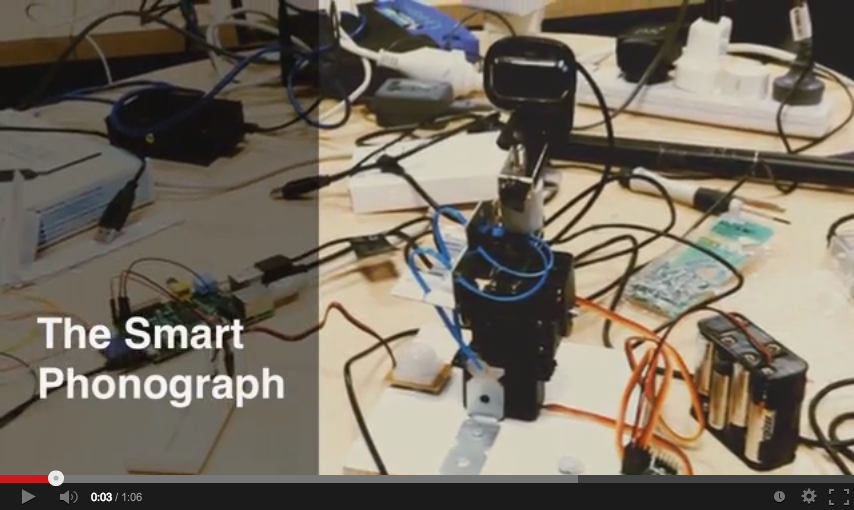
\includegraphics[width=\textwidth]{graphs/youtube.png}
}
\end{center}
See the video here: \url{http://www.youtube.com/watch?v=hckEBpT1VcU}



\subsection{Peer Review Summary}

The reviews from our classmates during the presentation were very positive. There have been encouragement from a number of students and our lab assistant to continue development of this project towards a commercially viable state. 

Some suggestions offered by the peer feedback forms as well as verbally included:

\begin{itemize}
    \item demonstrate the inter workings of the RPis (a behind-the-scenes view of sorts) through a streaming debug activity to an external monitor
    \item debug audio monitoring capability
    \item move to a better spec ARM board such as the Beagleboard to improve the performance of face detection
\end{itemize}


\subsection{Self Reflection / Lessons Learned}

Although we had a talented group, each individual team member took something away from this project.

\subsubsection{Val}

Having never worked with a Raspberry Pi before, I found the project quite enlightening, particularly in understanding the lower-level hardware interfacing through GPIO pins. 

The project also provided an awesome opportunity for me to learn off the other team members concepts and techniques I would otherwise encounter only as theory. It's been great to have such a wide knowledge base to draw upon when working towards troubleshooting and resolving hardware and software issues.

The work involving the servos and the Pololu servo controller was also the first time I had a chance to prototype a hardware device library from API documentation, which has subsequently greatly increased my confidence in own abilities.

Lastly, being required to work on a resource constrained device (Raspberry Pi) has really highlighted the value of measurement and optimisation of system performance, which provided real-world context a lot of the topics covered during our lectures.

\subsubsection{Alfred}

During the lab, I learnt how to use linux command, and how to use cross-complier to build a linux image.

I used a lot multi-threading programming, as a result of that I am now quiet familiar with Synchronisation in a linux way. In addition, the face detection had requirement on memory management, so I spent a long time to investigate how to implement this in C++. Also, the message dispatch helped me understand about how to schedule jobs.

Finally, thanks for Neil and Val, they help me a lot in this project. This is definitely the most successful group work for me while at RMIT.


\subsubsection{Neil}

This project gave me an excellent opportunity to try a lot of new things. Working on the \rpi\xspace and building a subject tracking system was something that I had never done before.


I had also never written a interface to device hardware before. It was very hard to debug but very satisfying once it was working. This also gave me the opportunity to expand my C and C++ experience.

The face detection was also very fun to work with. It was surprising easy to program and it has given me ideas for other potential projects where I could use this.


As a team I think we functioned very well. I normally try to avoid teamwork but our collection of skills and determination meant we delivered a project of a high standard.


Finally, this projec also gave me a chance to create two new open source projects. While researching how to interact with our hardware I found very little code examples available. In an effort to help others, I decided to open source hardware based components of the project.


\subsection{Description of how each learning objective is addressed}


Over the course of the project development, this team have made significant leaps in their knowledge of computer-hardware interfacing, operating system level functionality and application optimisation in a resource constrained environment. This section highlights how various learning objectives of the OSP course have been met.
 
\subsubsection{Learning Objective 1}
For the duration of this project, all of our ongoing development code has been managed through Github to ensure team members were always using the latest stable code when working on their assigned tasks.

With the face detection (computer vision) generating major CPU load when running on the Raspberry Pi, the team has gone through a significant amount of iterations of the functionality in order to achieve real-time response to the enviroment.


For efficiency during the initial development stages, most hardware interface interaction (e.g. servo controller, PIR sensor etc.) were prototyped using the Python programming language, and later ported into C when performance optimisation was required.


Debugging and performance has been used extensively over the course of the project for both hardware and software components. For Python, Pudb was the debugger of choice. For C/C++ Instruments and LLDB/GDB were utilised. On the hardware side, servo controller built-in error-checking was utilised for all communication to ensure hardware errors were caught and dealt with.

\textcolor{red}{TODO: Open sourced project to show mastery: https://github.com/neilang/pir-monitor}
\textcolor{red}{TODO: Open sourced project to show mastery: https://github.com/neilang/maestro-wrapper}


 
\subsubsection{Learning Objective 2}

\textcolor{orange}{Val, are you working on this learning objective?}

\subsubsection{Learning Objective 3}

\textcolor{orange}{Val, are you working on this learning objective?}

\subsubsection{Learning Objective 4}

\textcolor{orange}{Val, are you working on this learning objective?}



\section{Assumptions and Dependencies}

\textcolor{red}{TODO: This is a confusing heading... perhaps we can review what we had in the project specification here?}


\section{General Constraints}

\section{Development Methodology}

\textcolor{red}{TODO: Discuss our background using agile and how we differ from SCRUM. Reinforce how we met learning objective 1 here.}


\subsection{Programming languages}

\textcolor{red}{TODO: Python for prototyping, C/C++ for performance.}


\subsection{Development tools}

\textcolor{red}{TODO: Vim, Xcode, Instruments. Mention Pi compile performance...}

\subsection{Collaboration tools}

There were three main collaboration tools we used to progress this project: GitHub, Email and face-to-face meetings.

\subsubsection{GitHub}

From the start we setup a private\footnote{Access to this repository is available upon request.} git repository hosted on GitHub to store all our experimentation, development and production code. Since our project specification and portfolio were typeset in \LaTeX, we were also able to version control that as well. For all other project documentation (such as development logs and bibliography) we took advantage of GitHub's built in wiki to store this information.

GitHub worked for us because git was a version control system we all wanted to use, it was a tool we were familiar with, and it made it easy to identify when a piece of work had been completed.

\subsubsection{Email}

As postgraduate students, we all had competing priorities with our time which meant that we could not work together in person regularly. It was also difficult to meet due to the amount of hardware involved. As a result we often worked in isolation with very defined tasks.

So for us email was key for effective communication and delegating tasks. Once a week a group message was used to talk about our progress and goals for the coming week.

\subsubsection{Face-to-face meetings}

Being all together at once was a rare occasion and we had only a total of five out-of-class-hours group meetings that we all attended. We used the time to visually demonstrate what we had achieved with our tasks and discuss arising issues. 

If another group member was assigned to take over a task (e.g. handing over code to be optimised or integrated), we used this time to instruct in detail how the prototype code worked or how the hardware had been configured. 

\section{Difficulties Encountered}

\textcolor{red}{TODO: Slow-ness, CPU, GPU, meeting, depth sensing, hardware issues, debugging, benchmarking.}


\section{Architecture}
\subsection{System Design including configuration}

\textcolor{orange}{Perhaps some hardware diagrams would work here?}

\subsection{Data Design}

\textcolor{red}{TODO: Drop this heading? I think we did in the project spec.}

\subsection{Program Design}


The software architecture for this project is basically a C/S (Client and Service) pattern. The server and client are connecting with Linux socket, using UDP protocol. The project has been divided into separated components, and after we build demo program for each part, we calculate the CPU usage, and than distribute the component into server and client.

In terms of components, they adopt messages to communicating with each other. That is to say, each component only cares about their own jobs, which improves the hoisin and independency for the system.

\textcolor{red}{TODO: Add communication digram here}


\subsubsection{Architecture Decisions}

\textcolor{red}{TODO: Alter table into description list because of LaTeX issues with large tables.}


%\begin{description}
%
%  \item[Communication - TCP vs UDP] \hfill \\
%      lorem ipsum.
%      
%  \item[Performance - Idle vs Multi-threaded] \hfill \\
%      lorem ipsum.
%
%  \item[Library - OpenCV vs Pi face detect library] \hfill \\
%      lorem ipsum.
%
%  \item[Thread communication - Pipeline vs Shared memory] \hfill \\
%      lorem ipsum.
%
%  \item[Memory - Instance every copy vs Copy on write] \hfill \\
%      lorem ipsum.
%      
%  \item[Message scheduling - FCFS vs Complex algorithm] \hfill \\
%      lorem ipsum.
%      
%\end{description}

\begin{center}
\begin{table}
\begin{tabular}{|p{0.3\textwidth}|p{0.2\textwidth}|p{0.5\textwidth}|}
    \hline
    \textbf{Aspects} & \textbf{Options} & \textbf{Decisions} \\ \hline
    
     Communication & 1. TCP \newline 2. UDP & 1. This is a small project that we only measure two PI communications, so the package loses shall happen in low possibility. \newline  2. In terms of complexity of communication, we do not need the message queue manages whether the message is delivered or not. \newline \textit{Option 2 adopted.
} \\ \hline

     Performance & 1. Idle \newline 2. Multiple threads & 1. There are brunches of components needs to wait communication messages to take next step. If we use idle function, it shall increase the queries between each component, dropping the system's cohesion. \newline  2. The worst case for face detection algorithm shall take a long time on detecting, dropping the system’s performance dramatically. \newline \textit{Option 2 adopted.
} \\ \hline

     Library & 1. Open CV \newline 2. PI face detection library & 1. Easy to debug on the laptop. \newline  2. Open CV library supports the USB camera, which can easily located on servo. \newline \textit{Option 1 adopted.
} \\ \hline
     
     Thread Communication & 1. Pipeline \newline 2. Sharing memory & 1. Sharing memory provides better performance on communication. \newline  2. There are too many components that need to communication, if we use pipeline, it shall increase the complex for the project and decrease the maintenance. \newline \textit{Option 2 adopted.
} \\ \hline
     
     Memory & 1. Instance every copy
 \newline 2. Copy on write & 1. All components may assess the message data. if every component create an instance, there shall be a lot memory waste for brunches of different instance for same object.
 \newline  2. Copy on write provides more performance; because it shall not spend too much time on copying the data form one object to another. \newline \textit{Option 2 adopted.
} \\ \hline

     Message scheduling & 1. FCFS \newline 2. More complex algorithms & 1. FCFS is easy to implement and maintain.
 \newline  2. This is an easy project, and every message may have same priority. \newline \textit{Option 1 adopted.
} \\ \hline

\end{tabular}
\end{table}
\end{center}


\textcolor{red}{TODO: Add sequence digram here}

\subsubsection{Sharing memory for threads communication}

All the threads have their own stack, but they shall share the heap memory. So we build all the service in heap memory. (use malloc) In addition,  in order for easy accessing from different threads, we allocate a pointer in static memory block that point to the heap. 

The code of Singleton is shown as below:

\textcolor{red}{TODO: INSERT CODE}


\subsubsection{Memory Scheduling}

The most different part for the message definition is that the length of the message does not know before it construct. However, we cannot create a big buffer because of the memory limited for the PI. As a result of that, I use a strategy only define 1 char array, and use malloc to increase the length dynamically.

The code of dynamical message length is shown as below:

\textcolor{red}{TODO: INSERT CODE}


\subsubsection{Copy on write}

PI has little memory size, so it is impossible to reallco memory for passing large frame data buffer that come from face detection frame. More specify, it turn to be waste of memory coping more than one instance of any kind of instance in the project. 

In order to reduce the usage of memory, we adopt the Copy on write strategy. This strategy only makes a copy when there is some modification on the object, and the most of time they shall only create a new pointer point to the original address.

The trade-off for this strategy is that it is no thread-safe, because more than one thread want to access the object when about to change the original data. However, in our project, all the processes, such as face detection and messages, are read-only process, which means that we do not have to consider race condition when we use this approach. 

The code of message is shown as below:


\textcolor{red}{TODO: INSERT CODE}

\subsubsection{Message serialization}

As the communication between server and client, we encode the message data into an array that uses '\textbackslash0' at the end. And the message array can also be encoded into message.

The code of message serialization is shown as below:

\textcolor{red}{TODO: INSERT CODE}


\subsubsection{Message queue class}

The message queue acts as the communication component in the system. All other components push message to the message queue and the dispatch messages to appropriate component. 

The most important functionality for message queue should be synchronization. That is to say, only one thread can push or pop message at the same time in order to prevent race condition. More specific, the message queue use conditional valuable to control the race condition. 

The core code of message queue is shown as below:

\textcolor{red}{TODO: INSERT CODE}


\subsubsection{FCFS strategy}

The code shows that we use the simplest strategy to scheduling the message, which means that when there is a message push into the message queue, the dispatching thread shall read the first message in the message queue send to the appropriate component to serve it. In addition, the dispatch thread shall be hinge up and wait when there are no messages in message queue.

The message shall be dispatched messages using design pattern: chain of responsibility. The process base on the message ID, which have been introduced in message protocol part. The dispatch component shall query message id and push the message to the serve components.

The core code of client message dispatching is shown as below:

\textcolor{red}{TODO: INSERT CODE}





\subsubsection{Software Design}

\textcolor{red}{TODO: rehash the structure we used in the project spec}


\subsubsection{Source code or patches for all original work.}


\textcolor{orange}{Val to provide patch files for OS configuration.}

\textcolor{red}{TODO: Add description to each source file.}


\subsubsection{Server Code}

\begin{lstlisting}[caption=basic-service.h,language=C++]
#ifndef __BASE_SERVICE_H__
#define __BASE_SERVICE_H__

#include "message.h"
#include "message_query.h"

class base_service {
public:

  virtual bool setUpService()  = 0;
  virtual void startMainLoop() = 0;
  virtual void stopMainLoop()  = 0;

  virtual void postMessage(Message *m)
  {
    MessageQuery::GetInstance()->pushMessage(m);
  }

  virtual void receiveMessage(const Message& m) = 0;
};

#endif
\end{lstlisting}





\begin{lstlisting}[caption=comm.h,language=C++]
#define LISTEN_THREAD 0
#define WRITE_THREAD  1
#define READ_THREAD   2
#define THREAD_NUM    3

#include <pthread.h>
#include "message_query.h"
#include "message.h"
#include <sys/socket.h>
#include <netinet/in.h>
#include <arpa/inet.h>
#include <stdio.h>
#include <stdlib.h>
#include <errno.h>
#include <string.h>
#include <time.h>
#include <unistd.h>

class Comm {
protected:

  struct sockaddr_in serv_addr;
  int server_socket;
  int client_socket;

  pthread_t threads[THREAD_NUM];
  int  thread_ids[THREAD_NUM];
  bool thread_running[THREAD_NUM];

public:

  MessageQuery *query;

public:

  Comm();
  ~Comm();

  void         createThreads();
  bool         isThreadRunning(int thread_index);

  int          sendMessage(Message *m);
  Message    * readMessage();
  virtual bool dispatchMessage(Message *m) = 0;
};

void         * writeThread(void *arg);
void         * readThread(void *arg);

\end{lstlisting}







\begin{lstlisting}[caption=comm.cpp,language=C++]
#include <sys/socket.h>
#include <netinet/in.h>
#include <arpa/inet.h>
#include <stdio.h>
#include <stdlib.h>
#include <errno.h>
#include <string.h>
#include <time.h>
#include <unistd.h>

#define BUFFER_SIZE 1024

#include <iostream>
using std::cout;        using std::endl;

#include "comm.h"

Comm::Comm()
{
  query = MessageQuery::GetInstance();
  memset(thread_running, 1, THREAD_NUM);
}

Comm::~Comm()
{}

void Comm::createThreads()
{
  thread_ids[WRITE_THREAD] = pthread_create(&threads[WRITE_THREAD],
                                            NULL,
                                            writeThread,
                                            this);

  thread_ids[READ_THREAD] = pthread_create(&threads[READ_THREAD],
                                           NULL,
                                           readThread,
                                           this);
}

bool Comm::isThreadRunning(int thread_index)
{
  return thread_running[thread_index];
}

int Comm::sendMessage(Message *m)
{
  void *p = m->messageData();

  write(client_socket, p, m->messageLength());
  free(p);
  return 0;
}

Message * Comm::readMessage()
{
  char buffer[BUFFER_SIZE] = { 0 };
  int  count               = 0;

  count         = read(client_socket, buffer, sizeof(buffer) - 1);
  buffer[count] = 0;
  Message *m = Message::createMessage(buffer);
  return m;
}

void* writeThread(void *arg)
{
  printf("write thread start\n");

  Comm *s = (Comm *)arg;
  char  buffer[BUFFER_SIZE];

  while (s->isThreadRunning(WRITE_THREAD))
  {
    memset(buffer, 0, BUFFER_SIZE);

    Message *m = MessageQuery::GetInstance()->popMessage();
    s->sendMessage(m);
    delete m;
  }
  return NULL;
}

void* readThread(void *arg)
{
  printf("read thread start\n");

  Comm *s = (Comm *)arg;

  while (s->isThreadRunning(READ_THREAD))
  {
    Message *m = s->readMessage();

    printf("%s\n", m->messageBodyData());

    if (s->dispatchMessage(m)) delete m;
  }
  return NULL;
}
\end{lstlisting}





\begin{lstlisting}[caption=face-detect.h,language=C++]
#include "singleton.h"
#include "base_service.h"
#include <string>
#include <opencv2/opencv.hpp>
using std::string;
using namespace cv;

struct face_detect_arg;
class Message;

class face_detect
  : public Singleton<face_detect>
    , public base_service {
  const char *strWindowName;
  const char *strCascadeClassifier;
  const int   nFrameWaitTime;

  bool isRunning;

  face_detect_arg *fd;

public:

  pthread_t face_main_thread;
  pthread_t face_detect_thread;
  const int nFrameWidth;
  const int nFrameHeight;

public:

  bool             isMainThreadRunning() const;
  const char     * getWindowName() const;
  face_detect_arg* getDetectArg();
  const int        getFrameWaitTime() const;
  const int        getFrameWidth() const;
  const int        getFrameHeight() const;

  pthread_t        getMainThread() const;
  pthread_t        getDetectThread() const;

public:

  face_detect();
  ~face_detect();

  virtual bool setUpService();
  virtual void startMainLoop();
  virtual void stopMainLoop();
  virtual void receiveMessage(const Message& m);

public:

  void       loadCascadeClassifier(const char        *strPath,
                                   CascadeClassifier *pc);
  CvCapture* createCaptureFrameCamera(int nCaptureIndex = -1);
  IplImage * captureFrame(CvCapture *pCapture);
};

struct face_detect_arg
{
  CascadeClassifier *pCvHaar;
  IplImage          *pImage;
  bool               bDetected;
  CvRect             rc;
  bool               threadRunning;
};

void * faceCaptureFunction(void *arg);
void * faceDetectFunction(void *arg);
CvRect detectFaceInImage(IplImage          *inputImg,
                         CascadeClassifier *cascade);

\end{lstlisting}








\begin{lstlisting}[caption=face-detect.cpp,language=C++]
#include <opencv2/opencv.hpp>
#include <string>
#include <iostream>
#include <vector>
#include <assert.h>
#include <pthread.h>
#include "face_detect.h"
#include "message.h"
#include "maestro.h"
#include <stdio.h>
using std::string;      using std::cout;
using std::endl;        using std::vector;
using std::cerr;
using namespace cv;

#define NA_FACE_MOVE_THRESHOLD 400
#define GUI_MODE 0

pthread_mutex_t mutex = PTHREAD_MUTEX_INITIALIZER;

#define FAILURE_CHECK(p, x)      \
  assert(p);                     \
  if (p == NULL)                 \
  {                              \
    std::cerr << x << std::endl; \
    exit(EXIT_FAILURE);          \
  }

face_detect::face_detect()
  : strWindowName("Face detection test")
    , strCascadeClassifier("lbpcascade_frontalface.xml")
    , nFrameWaitTime(33)
    , nFrameWidth(320)
    , nFrameHeight(240)
    , isRunning(false)
{}

face_detect::~face_detect()
{}

bool face_detect::setUpService()
{
  fd          = (face_detect_arg *)malloc(sizeof(face_detect_arg));
  fd->pCvHaar = new CascadeClassifier();
  loadCascadeClassifier(strCascadeClassifier, fd->pCvHaar);

  fd->pImage        = NULL;
  fd->threadRunning = true;
  fd->bDetected     = false;

  return true;
}

void face_detect::startMainLoop()
{
  isRunning = true;
  pthread_create(&face_main_thread, NULL, faceCaptureFunction, (void *)_instance);

  //	faceCaptureFunction((void*)this);
}

void face_detect::stopMainLoop()
{
  isRunning         = false;
  fd->threadRunning = false;
}

void face_detect::receiveMessage(const Message& m)
{
  // TODO: handle the message ...
}

void face_detect::loadCascadeClassifier(const char        *strPath,
                                        CascadeClassifier *pc)
{
  FAILURE_CHECK(pc, "Conldn't load classifier");

  if (!pc->load(strPath))
  {
    std::cerr << "Conldn't load classifier" << endl;
    exit(EXIT_FAILURE);
  }
}

CvCapture * face_detect::createCaptureFrameCamera(int nCaptureIndex)
{
  CvCapture *p = cvCaptureFromCAM(nCaptureIndex);

  FAILURE_CHECK(p, "Init Capture Failed");

  if (!cvGrabFrame(p))
  {
    std::cerr << "Conldn't GrabFrame" << std::endl;
    exit(EXIT_FAILURE);
  }

  cvSetCaptureProperty(p, CV_CAP_PROP_FRAME_WIDTH,  nFrameWidth);
  cvSetCaptureProperty(p, CV_CAP_PROP_FRAME_HEIGHT, nFrameHeight);
  cvSetCaptureProperty(p, CV_CAP_PROP_FPS,          5);

  return p;
}

IplImage * face_detect::captureFrame(CvCapture *pCapture)
{
  IplImage *p = cvQueryFrame(pCapture);

  FAILURE_CHECK(p, "Error: cvQueryFrame failed");

  return p;
}

CvRect detectFaceInImage(IplImage *inputImg, CascadeClassifier *cascade)
{

  CvSize minFeatureSize = cvSize(80, 80);

  int flags = CV_HAAR_FIND_BIGGEST_OBJECT | CV_HAAR_DO_ROUGH_SEARCH;

  float search_scale_factor = 1.1f;

  IplImage *detectImg = inputImg;

  if (detectImg->nChannels > 1)
  {
    CvSize size       = cvSize(detectImg->width, detectImg->height);
    IplImage *greyImg = cvCreateImage(size, IPL_DEPTH_8U, 1);
    cvCvtColor(detectImg, greyImg, CV_BGR2GRAY);
    detectImg = greyImg;
  }

  vector<Rect> rects;
  cascade->detectMultiScale(detectImg,
                            rects,
                            search_scale_factor,
                            3,
                            flags,
                            minFeatureSize);

  int nFaces = rects.size();

  CvRect rc = cvRect(-1, -1, -1, -1);

  if (nFaces > 0)
  {
    rc = cvRect(rects[0].x, rects[0].y, rects[0].width, rects[0].height);
  }

  if (detectImg->nChannels > 1) cvReleaseImage(&detectImg);

  return rc;
}

double euclideanDistance(CvPoint pt1, CvPoint pt2) {
  double x = pt1.x - pt2.x;
  double y = pt1.y - pt2.y;
  double dist;

  dist = pow(x, 2) + pow(y, 2);
  return dist;
}

void* faceCaptureFunction(void *arg)
{
  face_detect *fdc    = (face_detect *)arg;
  face_detect_arg *fd = fdc->getDetectArg();

  CvCapture *pCapture = fdc->createCaptureFrameCamera();

  IplImage *src =  cvQueryFrame(pCapture);

  pthread_create(&(fdc->face_detect_thread), NULL, faceDetectFunction,
                 (void *)fd);

  float screenDivisions = 2.6;

  Point rightPt2  = Point(fdc->nFrameWidth / screenDivisions,
                          fdc->nFrameHeight - 1);
  Point leftPt1   = Point(fdc->nFrameWidth - (fdc->nFrameWidth / screenDivisions),
                          0);
  Point topPt2    = Point(fdc->nFrameWidth - 1,
                          fdc->nFrameHeight / screenDivisions);
  Point bottomPt1 =
    Point(0, fdc->nFrameHeight - (fdc->nFrameHeight / screenDivisions));

  Maestro *maestro = Maestro::GetInstance();
  maestro->goHome(maestro->horizontalServo);
  maestro->goHome(maestro->verticalServo);
      usleep(1);

  CvPoint lastFace;
  lastFace.x = fdc->nFrameWidth / 2.0;
  lastFace.y = fdc->nFrameHeight / 2.0;

  CvRect rc;
  bool   bDetected = false;

  while (fdc->isMainThreadRunning())
  {
    IplImage *pImg = cvQueryFrame(pCapture);

    if (!pImg)
    {
      std::cerr << "Query Frame Failed" << endl;
      usleep(1000);
      continue;
    }

    assert(pImg);
    pthread_mutex_lock(&mutex);
    fd->pImage = pImg;
    bDetected  = fd->bDetected;
    rc         = fd->rc;
    pthread_mutex_unlock(&mutex);

    CvPoint facePoint;
    facePoint.x = 0;
    facePoint.y = 0;

    if (bDetected)
    {
      CvPoint p1 = cvPoint(rc.x, rc.y);
      CvPoint p2 = cvPoint(rc.x + rc.width, rc.y + rc.height);
      cvRectangle(pImg, p1, p2, CV_RGB(0, 255, 0), 5, 8);

      facePoint.x = rc.x + (rc.width / 2.0f);
      facePoint.y = rc.y + (rc.height / 2.0f);

        printf("Face Detected\n");
    }

    if ((facePoint.x > 0) && (facePoint.y > 0)) {
      double dist = euclideanDistance(facePoint, lastFace);

      if ((dist > 0) && (dist < NA_FACE_MOVE_THRESHOLD))
      {
        printf("send rotate command\n");

        if (facePoint.x < rightPt2.x) maestro->stepUp(maestro->horizontalServo);
        else if (facePoint.x > leftPt1.x) maestro->stepDown(
            maestro->horizontalServo);

        if (facePoint.y < topPt2.y) maestro->stepUp(maestro->verticalServo);

        else if (facePoint.y > bottomPt1.y) maestro->stepDown(
            maestro->verticalServo);
      }

      lastFace.x = facePoint.x;
      lastFace.y = facePoint.y;
    }

    if (cvWaitKey(fdc->getFrameWaitTime()) == 27) fdc->stopMainLoop();

    usleep(1);
  }

  cvReleaseCapture(&pCapture);
  return NULL;
}

void* faceDetectFunction(void *arg)
{
  face_detect_arg *fd = (face_detect_arg *)arg;

  while (fd->threadRunning)
  {
    if (fd->pImage == NULL)
    {
      continue;
    }

    pthread_mutex_lock(&mutex);
    IplImage *pImg = fd->pImage;
    pthread_mutex_unlock(&mutex);

    CvRect rc = detectFaceInImage(pImg, fd->pCvHaar);

    if (rc.x != -1)
    {
      pthread_mutex_lock(&mutex);
      fd->bDetected = true;
      fd->rc        = rc;
      pthread_mutex_unlock(&mutex);
    }
    else
    {
      pthread_mutex_lock(&mutex);
      fd->bDetected = false;
      pthread_mutex_unlock(&mutex);
    }
  }

  return NULL;
}

bool face_detect::isMainThreadRunning() const
{
  return isRunning;
}

const char * face_detect::getWindowName() const
{
  return strWindowName;
}

face_detect_arg * face_detect::getDetectArg()
{
  return fd;
}

pthread_t face_detect::getMainThread() const
{
  return face_main_thread;
}

pthread_t face_detect::getDetectThread() const
{
  return face_detect_thread;
}

const int face_detect::getFrameWaitTime() const
{
  return nFrameWaitTime;
}

const int face_detect::getFrameWidth() const
{
  return nFrameWidth;
}

const int face_detect::getFrameHeight() const
{
  return nFrameHeight;
}

\end{lstlisting}





\begin{lstlisting}[caption=maestro.h,language=C++]
#ifndef __maestro__
#define __maestro__

#include <iostream>
#include <string>
#include <stdio.h>
#include <unistd.h>
#include <fcntl.h>
#include <termios.h>

#include "singleton.h"
#include "base_service.h"

// Source:
// http://stackoverflow.com/questions/134569/c-exception-throwing-stdstring
struct MaestroException : public std::exception
{
  std::string s;
  MaestroException(std::string ss) : s(ss) {}

  ~MaestroException() throw() {}

  const char* what() const throw() {
    return s.c_str();
  }
};

#ifndef __servo__
# define __servo__

class Servo {
private:

  unsigned char  _channel;
  unsigned int   _min;
  unsigned int   _max;
  unsigned short _pos;
  unsigned short _home;

public:

  Servo(unsigned char c, unsigned int mn, unsigned int mx,
        unsigned int hm) : _channel(c), _min(mn), _max(mx), _home(hm) {}

  unsigned char getChannel() {
    return _channel;
  }

  unsigned short getHome() {
    return _home;
  }

  unsigned short getMin() {
    return _min;
  }

  unsigned short getMax() {
    return _max;
  }

  unsigned short getPos() {
    return _pos;
  }

  void setPos(unsigned short p) {
    _pos = p;
  }
};

#endif /* defined(__servo__) */

#ifdef __APPLE__
# define NA_DEVICE "/dev/cu.usbmodem00065291"
#else
# define NA_DEVICE "/dev/ttyACM0"
#endif // ifdef __APPLE__

class Maestro
  : public Singleton<Maestro>
    , public base_service {
private:

  const char *_device;
  int         _fd;

public:

  Servo *horizontalServo;
  Servo *verticalServo;

public:

  Maestro() : _device(NA_DEVICE) {}

  ~Maestro() {
    close(_fd);
  }

  int          getError(Servo *servo);
  int          goHome(Servo *);
  int          getPosition(Servo *);
  int          setPosition(Servo    *,
                           unsigned short);
  int          stepUp(Servo *);
  int          stepDown(Servo *);

  virtual bool setUpService();
  virtual void startMainLoop();
  virtual void stopMainLoop();
  virtual void receiveMessage(const Message& m);

private:

  void openDevice();
};

#endif // ifndef __maestro__

\end{lstlisting}





\begin{lstlisting}[caption=maestro.cpp,language=C++]
#include "maestro.h"
#define NA_STEP_VALUE 150

int Maestro::goHome(Servo *servo) {
  unsigned char command[] = { 0xA2, servo->getChannel() };

  if (write(_fd, command, sizeof(command)) == -1) {
    perror("error writing");
    return -1;
  }

  servo->setPos(servo->getHome());

  return 0;
}

int Maestro::getPosition(Servo *servo) {
  return (int)servo->getPos();
}

int Maestro::setPosition(Servo *servo, unsigned short target) {
  if (target > servo->getMax()) target = servo->getMax();

  if (target < servo->getMin()) target = servo->getMin();
  unsigned char command[] =
  { 0x84, servo->getChannel(), static_cast<unsigned char>(target & 0x7F),
    static_cast<unsigned char>(target >> 7 & 0x7F) };

  if (write(_fd, command, sizeof(command)) == -1) {
    perror("error writing");
    return -1;
  }

  servo->setPos(target);
  return 0;
}

int Maestro::stepUp(Servo *servo) {
  return setPosition(servo, getPosition(servo) + NA_STEP_VALUE);
}

int Maestro::stepDown(Servo *servo) {
  return setPosition(servo, getPosition(servo) - NA_STEP_VALUE);
}

#define KEYCONTROL 0

#if KEYCONTROL
# include <termios.h>
# include <unistd.h>
#endif // if KEYCONTROL

void Maestro::openDevice()
{
  _fd = open(_device, O_RDWR | O_NOCTTY);

  if (_fd == -1) {
    perror(_device);
    throw MaestroException("Invalid Device");
  }
}

bool Maestro::setUpService()
{
  openDevice();
  horizontalServo = new Servo(0, 3968, 9216, 6104);
  verticalServo   = new Servo(1, 3968, 9216, 8220);

  this->goHome(horizontalServo);
  this->goHome(verticalServo);
}

void Maestro::startMainLoop()
{}

void Maestro::stopMainLoop()
{}

void Maestro::receiveMessage(const Message& m)
{}

#undef NA_STEP_VALUE
\end{lstlisting}





\begin{lstlisting}[caption=main-server.cpp,language=C++]
#include "server.h"

int main(int argc, char **argv)
{
  Server *s = Server::GetInstance();

  s->setUpService();
  s->startMainLoop();

  return 0;
}
\end{lstlisting}





\begin{lstlisting}[caption=message.h,language=C++]
#ifndef __MESSAGE_H__
#define __MESSAGE_H__

#include <string>
using std::string;

#define TEST 0

enum message_id
{
  M_START = 0,
  M_END,
  M_DETECTED,
  M_UNDETECTED,

  M_PIR_DETECTED = 100,
  M_PIR_UN_DETECTED,

  M_BEGIN_AUDIO_RECORDING = 200,
  M_END_AUDIO_RECORDING,
};

enum message_handle_proxy
{
  proxy_server = 0,
  proxy_client,
};

struct message_head
{
  int mh_id;
  int mh_size;
  int mh_handle_proxy;
  int mh_reserve;
};

struct message_body
{
  int  mb_len;
  char mb_data[1];
};

struct message
{
  message_head *head;
  message_body *body;
};

class Server;

class Message {
  friend class Server;
#if TEST

public:

#endif // if TEST
  message *_impl;

public:

  Message();
  Message(const Message& other);
  Message& operator=(const Message& rhs);
  Message(void *data, int size);
  ~Message();

public:

  void            initMessage(int    id,
                              string message_data);
  int             messageLength() const;
  void          * messageData() const;
  char          * messageBodyData() const;
  int             getMessageHandleProxy(int id);

  static Message* createMessage(void *data);
};

#endif

\end{lstlisting}





\begin{lstlisting}[caption=message.cpp,language=C++]
#include "message.h"
#include <stdlib.h>
#include <stdio.h>
#include <string.h>

Message::Message()
{
  _impl       = new message();
  _impl->head = new message_head();
  _impl->body = (message_body *)malloc(sizeof(message_body));
}

Message::Message(const Message& other)
{
  _impl       = new message();
  _impl->head = new message_head();
  _impl->body = (message_body *)malloc(sizeof(message_body));

    memcpy(_impl, other._impl, sizeof(message));
}

Message& Message::operator=(const Message& rhs)
{
  if (&rhs != this)
  {
    _impl       = new message();
    _impl->head = new message_head();
    _impl->body = (message_body *)malloc(sizeof(message_body));

    memcpy(_impl, rhs._impl, sizeof(message));
  }

  return *this;
}

Message::~Message()
{
  delete _impl->head;
  delete _impl->body;
  delete _impl;
}

Message * Message::createMessage(void *data)
{
  Message *m = new Message();

  int *p = (int *)data;

  m->_impl->head->mh_id           = *(p + 0);
  m->_impl->head->mh_size         = *(p + 1);
  m->_impl->head->mh_handle_proxy = *(p + 2);
  m->_impl->head->mh_reserve      = *(p + 3);
  char *c   = (char *)((p + 4) + 1);
  int   len = strlen(c);
  m->_impl->body         = (message_body *)malloc(
    sizeof(char) * (len + 1) + sizeof(int));
  m->_impl->body->mb_len = *(p + 4);
    memcpy(m->_impl->body->mb_data, c, len);
  m->_impl->body->mb_data[len] = 0;

  return m;
}

void Message::initMessage(int id, string message_data)
{
  _impl->head->mh_id = id;

  _impl->head->mh_handle_proxy = getMessageHandleProxy(id);
  _impl->head->mh_reserve      = 0;

  _impl->body = (message_body *)malloc(sizeof(int) +
                                       sizeof(char) * (message_data.size() + 1));
  _impl->body->mb_len = message_data.size();
    memcpy(_impl->body->mb_data, message_data.c_str(), message_data.size());
  *(_impl->body->mb_data + message_data.size()) = 0;

  _impl->head->mh_size = sizeof(message_head) + sizeof(int)
                         + sizeof(char) * (message_data.size() + 1);
}

int Message::messageLength() const
{
  return _impl->head->mh_size;
}

void * Message::messageData() const
{
  void *p = malloc(messageLength());

  memset(p, 0, messageLength());
  memcpy(p, _impl->head, sizeof(message_head));
  int *pi = ((int *)p + 4);
  *pi = _impl->body->mb_len;
  char *c = (char *)(pi + 1);
  memcpy(c, _impl->body->mb_data, _impl->body->mb_len);
  c[_impl->body->mb_len] = 0;
  return p;
}

char * Message::messageBodyData() const
{
  return _impl->body->mb_data;
}

int Message::getMessageHandleProxy(int id)
{
  int reVal = -1;

  switch (id)
  {
  case M_START:
  case M_END:
  case M_DETECTED:
  case M_UNDETECTED:
  case M_PIR_DETECTED:
  case M_PIR_UN_DETECTED:
    reVal = proxy_server;
    break;

  case M_BEGIN_AUDIO_RECORDING:
  case M_END_AUDIO_RECORDING:
    reVal = proxy_client;
    break;
  }
  return reVal;
}
\end{lstlisting}





\begin{lstlisting}[caption=message-query.cpp,language=C++]
#ifndef __MESSAGE_QUERY_H__
#define __MESSAGE_QUERY_H__

#include <list>
#include <pthread.h>
#include "singleton.h"
using std::list;

class Message;

class MessageQuery : public Singleton<MessageQuery>{
  list<Message *> _query;

  pthread_mutex_t _mutex;
  pthread_cond_t  _con;

public:

  MessageQuery();
  ~MessageQuery();

  void     pushMessage(Message *m);
  Message* popMessage();

};

#endif

\end{lstlisting}





\begin{lstlisting}[caption=message-query.cpp,language=C++]
#include "message_query.h"
#include "message.h"

MessageQuery::MessageQuery()
{
  pthread_mutex_init(&_mutex, NULL);
  pthread_cond_init(&_con, NULL);
}

MessageQuery::~MessageQuery()
{
  pthread_mutex_destroy(&_mutex);
  pthread_cond_destroy(&_con);
}

void MessageQuery::pushMessage(Message *m)
{
  pthread_mutex_lock(&_mutex);
  _query.push_back(m);
  pthread_cond_signal(&_con);
  pthread_mutex_unlock(&_mutex);
}

Message * MessageQuery::popMessage()
{
  pthread_mutex_lock(&_mutex);

  while (_query.empty()) pthread_cond_wait(&_con, &_mutex);

  Message *reVal = _query.front();
  _query.pop_front();
  pthread_mutex_unlock(&_mutex);
  return reVal;
}
\end{lstlisting}






\begin{lstlisting}[caption=pir-monitor.h,language=C++]
#ifndef __PIR_MONITOR_H__
#define __PIR_MONITOR_H__

#include "singleton.h"
#include "base_service.h"
#include <time.h>

class pir_monitor
  : public Singleton<pir_monitor>
    , public base_service {
  bool   isRunning;
  time_t last_sensor;

public:

  pir_monitor();
  ~pir_monitor();

  virtual bool setUpService();
  virtual void startMainLoop();
  virtual void stopMainLoop();
  virtual void receiveMessage(const Message& m);
};

#endif
\end{lstlisting}






\begin{lstlisting}[caption=pir-monitor.cpp,language=C++]
#include "pir_monitor.h"
#include "face_detect.h"
#include <bcm2835.h>
#include <stdio.h>
#include <stdlib.h>
#include <time.h>
#include <string.h>

#define NA_PIN RPI_GPIO_P1_07
#define NA_POLL_DELAY 33
#define NA_PIN_STILL_VALUE 1

pir_monitor::pir_monitor()
{}

pir_monitor::~pir_monitor()
{
  bcm2835_close();
}

bool pir_monitor::setUpService()
{
  bool reVal = true;

  if (!bcm2835_init()) {
    printf("Can't access hardware, did you use sudo?\n");
    exit(EXIT_FAILURE);
    reVal = false;
  }

  bcm2835_gpio_fsel(NA_PIN, BCM2835_GPIO_FSEL_INPT);

  bcm2835_gpio_set_pud(NA_PIN, BCM2835_GPIO_PUD_UP);

  return reVal;
}

void pir_monitor::stopMainLoop()
{
  isRunning = false;
}

void pir_monitor::startMainLoop()
{
  uint8_t value = NA_PIN_STILL_VALUE;

  time(&last_sensor);
  isRunning = true;

  while (isRunning)
  {
    value = bcm2835_gpio_lev(NA_PIN);

    if (value != NA_PIN_STILL_VALUE)
    {
        printf("dectect movement\n");
      face_detect *fd = face_detect::GetInstance();

      if (!fd->isMainThreadRunning())
      {
        printf("begin face detection");
        fd->startMainLoop();
      }

      time(&last_sensor);

      // Message to start Recording
      char buffer[100];
      memset(buffer, 0, 100);
      sprintf(buffer, "detected: %d\n", (int)last_sensor);
      Message *m = new Message();
      m->initMessage(M_BEGIN_AUDIO_RECORDING, buffer);
      this->postMessage(m);
    }
    else
    {
      time_t new_sensor;
      time(&new_sensor);

      if (difftime(new_sensor, last_sensor) > 30)
      {
        face_detect::GetInstance()->stopMainLoop();

        // Message to stop Recording
        char buffer[100];
        memset(buffer, 0, 100);
        sprintf(buffer, "detected: %d\n", (int)new_sensor);
        Message *m = new Message();
        m->initMessage(M_END_AUDIO_RECORDING, buffer);
        this->postMessage(m);
      }
    }

    delay(NA_POLL_DELAY);
  }

}

void pir_monitor::receiveMessage(const Message& m)
{
}

#undef NA_PIN
#undef NA_POLL_DELAY
#undef NA_PIN_STILL_VALUE

\end{lstlisting}






\begin{lstlisting}[caption=server.h,language=C++]
#include "comm.h"
#include "singleton.h"
#include "base_service.h"

class Server : public Comm
               , public Singleton<Server>
               , public base_service {
  bool isRunning;

public:

  Server();
  ~Server();

  virtual bool setUpService();
  virtual void startMainLoop();
  virtual void stopMainLoop();
  virtual void receiveMessage(const Message& m);
  virtual bool dispatchMessage(Message *m);

private:

  void startPirDetect();
  void startServer();
};

\end{lstlisting}






\begin{lstlisting}[caption=server.cpp,language=C++]
#include "server.h"
#include <sys/socket.h>
#include <netinet/in.h>
#include <arpa/inet.h>
#include <stdio.h>
#include <stdlib.h>
#include <errno.h>
#include <string.h>
#include <time.h>
#include <unistd.h>

#include "face_detect.h"
#include "pir_monitor.h"
#include "maestro.h"

Server::Server()
  : isRunning(true)
{}

Server::~Server()
{}

void Server::startPirDetect()
{
  pir_monitor::GetInstance()->startMainLoop();
}

void Server::startServer()
{
  client_socket = accept(server_socket, (struct sockaddr *)NULL, NULL);
}

bool Server::setUpService()
{
  server_socket = socket(AF_INET, SOCK_STREAM, 0);
  memset(&serv_addr, 0, sizeof(struct sockaddr_in));

  serv_addr.sin_family      = AF_INET;
  serv_addr.sin_addr.s_addr = htonl(INADDR_ANY);
  serv_addr.sin_port        = htons(9999);

  bind(server_socket, (struct sockaddr *)&serv_addr, sizeof(serv_addr));
  listen(server_socket, 10);

  startServer();
  createThreads();

  pir_monitor::GetInstance()->setUpService();

  face_detect::GetInstance()->setUpService();

  Maestro::GetInstance()->setUpService();

  return true;
}

void Server::startMainLoop()
{
  while (isRunning)
  {
    startPirDetect();
    usleep(10);
  }
}

void Server::stopMainLoop()
{
  isRunning = false;
}

void Server::receiveMessage(const Message& m)
{
}

bool Server::dispatchMessage(Message *m)
{
  bool bHandle = false;

  if (m->_impl->head->mh_handle_proxy == proxy_server)
  {
    bHandle = true;
  }
  else this->sendMessage(m);

  return bHandle;
}

\end{lstlisting}






\begin{lstlisting}[caption=singleton.h,language=C++]
#ifndef __SINGLETON_H__
#define __SINGLETON_H__

template<typename T>
class Singleton {
protected:

  static T *_instance;

public:

  static T* GetInstance()
  {
    if (!_instance) _instance = new T();

    return _instance;
  }
};

template<typename T>
T * Singleton<T>::_instance = 0;

#endif
\end{lstlisting}






\begin{lstlisting}[caption=.cpp,language=C++]
\end{lstlisting}





\subsubsection{Client Code}

\begin{lstlisting}[caption=basic-service.h,language=C++]
#ifndef __BASE_SERVICE_H__
#define __BASE_SERVICE_H__

#include "message.h"
#include "message_query.h"

class base_service {
public:

  virtual bool setUpService()  = 0;
  virtual void startMainLoop() = 0;
  virtual void stopMainLoop()  = 0;

  virtual void postMessage(Message *m)
  {
    MessageQuery::GetInstance()->pushMessage(m);
  }

  virtual void receiveMessage(const Message& m) = 0;
};

#endif
\end{lstlisting}




\begin{lstlisting}[caption=client.h,language=C++]
#include "comm.h"
#include "singleton.h"
#include "base_service.h"

class Client : public Comm
               , public Singleton<Client>
               , public base_service {
  pthread_t input_thread;
  bool isRecording;

public:

  bool isRunning;

  Client();
  ~Client();

  virtual bool setUpService();
  virtual void startMainLoop();
  virtual void stopMainLoop();
  virtual void receiveMessage(const Message& m);
  virtual bool dispatchMessage(Message *m);

private:

  void connectToServer();
  int  sendCommand(char *);
  void startAudioRecording();
  void stopAudioRecording();
};
\end{lstlisting}





\begin{lstlisting}[caption=client.cpp,language=C++]
#include "client.h"
#include <sys/socket.h>
#include <netinet/in.h>
#include <arpa/inet.h>
#include <stdio.h>
#include <stdlib.h>
#include <errno.h>
#include <string.h>
#include <time.h>
#include <unistd.h>
#include <stdio.h>
#include <stdlib.h>
#include <fcntl.h>
#include <sys/types.h>
#include <sys/stat.h>

#define HOSTNAME "192.168.1.126"

Client::Client()
  : isRecording(false)
    , isRunning(true)
{}

Client::~Client()
{
  printf("shut down recording");
  sendCommand("shutdown\r");
}

void Client::connectToServer()
{
  if (connect(client_socket, (struct sockaddr *)&serv_addr,
              sizeof(serv_addr)) < 0)
  {
    printf("\n Error: Connect Failed\n");
    exit(1);
  }
}

void* inputFunction(void *arg)
{
  Client *client = (Client *)arg;

  char c;

  scanf("%c", &c);

  if (c == 27) client->isRunning = false;

  return NULL;
}

bool Client::setUpService()
{
  memset(&serv_addr, 0, sizeof(struct sockaddr_in));

  if ((client_socket = socket(AF_INET, SOCK_STREAM, 0)) < 0)
  {
    printf("\n Error: Could not create socket \n");
  }

  serv_addr.sin_family = AF_INET;
  serv_addr.sin_port   = htons(9999);

  if (inet_pton(AF_INET, HOSTNAME, &serv_addr.sin_addr) <= 0)
  {
    printf("\n Error: Connect Failed \n");
    exit(1);
  }

  connectToServer();
  createThreads();


  pthread_create(&input_thread, NULL, inputFunction, (void *)this);

  // TODO: Voice Recode
  return true;
}

void Client::startMainLoop()
{
  while (isRunning)
  {}
}

void Client::stopMainLoop()
{
  isRunning = false;
}

void Client::receiveMessage(const Message& m)
{}

bool Client::dispatchMessage(Message *m)
{
  bool bHandle = false;

  if (m->_impl->head->mh_handle_proxy == proxy_client)
  {
    printf("client dispatching message");

    if (m->_impl->head->mh_id == M_BEGIN_AUDIO_RECORDING) startAudioRecording();

    else if (m->_impl->head->mh_id == M_END_AUDIO_RECORDING) stopAudioRecording();


    bHandle = true;
  }
  else this->sendMessage(m);

  return bHandle;
}

#define FIFO_NAME "/tmp/osp.fifo"

int Client::sendCommand(char *cmd) {
  int fd = open(FIFO_NAME, O_WRONLY);

  if (write(fd, cmd, strlen(cmd)) == -1) {
    perror(":(");
    return -1;
  }

  close(fd);

  return 1;
}

void Client::startAudioRecording()
{
  printf("start Audio Recording\n");

  if (!isRecording)
  {
    sendCommand("start\r");
    isRecording = true;
  }
}

void Client::stopAudioRecording()
{
  printf("start Audio Recording\n");

  if (isRecording)
  {
    sendCommand("stop\r");
    isRecording = false;
  }
}
\end{lstlisting}





\begin{lstlisting}[caption=comm.h,language=C++]
#define LISTEN_THREAD 0
#define WRITE_THREAD  1
#define READ_THREAD   2
#define THREAD_NUM    3

#include <pthread.h>
#include "message_query.h"
#include "message.h"
#include <sys/socket.h>
#include <netinet/in.h>
#include <arpa/inet.h>
#include <stdio.h>
#include <stdlib.h>
#include <errno.h>
#include <string.h>
#include <time.h>
#include <unistd.h>

class Comm {
protected:

  struct sockaddr_in serv_addr;
  int server_socket;
  int client_socket;

  pthread_t threads[THREAD_NUM];
  int  thread_ids[THREAD_NUM];
  bool thread_running[THREAD_NUM];

public:

  MessageQuery *query;

public:

  Comm();
  ~Comm();

  void         createThreads();
  bool         isThreadRunning(int thread_index);

  int          sendMessage(Message *m);
  Message    * readMessage();
  virtual bool dispatchMessage(Message *m) = 0;
};

void         * writeThread(void *arg);
void         * readThread(void *arg);

\end{lstlisting}





\begin{lstlisting}[caption=comm.cpp,language=C++]
#include <sys/socket.h>
#include <netinet/in.h>
#include <arpa/inet.h>
#include <stdio.h>
#include <stdlib.h>
#include <errno.h>
#include <string.h>
#include <time.h>
#include <unistd.h>

#define BUFFER_SIZE 1024

#include <iostream>
using std::cout;        using std::endl;

#include "comm.h"

Comm::Comm()
{
  query = MessageQuery::GetInstance();
  memset(thread_running, 1, THREAD_NUM);
}

Comm::~Comm()
{}

void Comm::createThreads()
{
  thread_ids[WRITE_THREAD] = pthread_create(&threads[WRITE_THREAD],
                                            NULL,
                                            writeThread,
                                            this);

  thread_ids[READ_THREAD] = pthread_create(&threads[READ_THREAD],
                                           NULL,
                                           readThread,
                                           this);
}

bool Comm::isThreadRunning(int thread_index)
{
  return thread_running[thread_index];
}

int Comm::sendMessage(Message *m)
{
  void *p = m->messageData();

  write(client_socket, p, m->messageLength());
  free(p);
  return 0;
}

Message * Comm::readMessage()
{
  char buffer[BUFFER_SIZE] = { 0 };
  int  count               = 0;

  count         = read(client_socket, buffer, sizeof(buffer) - 1);
  buffer[count] = 0;
  Message *m = Message::createMessage(buffer);
  return m;
}

void* writeThread(void *arg)
{
  Comm *s = (Comm *)arg;
  char  buffer[BUFFER_SIZE];

  while (s->isThreadRunning(WRITE_THREAD))
  {
    memset(buffer, 0, BUFFER_SIZE);
    Message *m = MessageQuery::GetInstance()->popMessage();
    s->sendMessage(m);
    delete m;
  }
  return NULL;
}

void* readThread(void *arg)
{
    printf("read thread start\n");

  Comm *s = (Comm *)arg;

  while (s->isThreadRunning(READ_THREAD))
  {
    Message *m = s->readMessage();
    printf("%s\n", m->messageBodyData());

    if (s->dispatchMessage(m)) delete(m);
  }
  return NULL;
}

\end{lstlisting}








\begin{lstlisting}[caption=main-client.cpp,language=C++]
#include "client.h"

int main(int argc, char **argv)
{
  Client *c = new Client();

  c->setUpService();
  c->startMainLoop();
  delete c;

  return 0;
}
\end{lstlisting}







\begin{lstlisting}[caption=message.h,language=C++]
#ifndef __MESSAGE_H__
#define __MESSAGE_H__

#include <string>
using std::string;

enum message_id
{
  M_START = 0,
  M_END,
  M_DETECTED,
  M_UNDETECTED,


  M_PIR_DETECTED = 100,
  M_PIR_UN_DETECTED,

  M_BEGIN_AUDIO_RECORDING = 200,
  M_END_AUDIO_RECORDING,
};

enum message_handle_proxy
{
  proxy_server,
  proxy_client,
};

struct message_head
{
  int mh_id;
  int mh_size;
  int mh_handle_proxy;
  int mh_reserve;
};

struct message_body
{
  int  mb_len;
  char mb_data[1];
};

struct message
{
  message_head *head;
  message_body *body;
};

class Client;

class Message {
  friend class Client;
  message *_impl;

public:

  Message();
  Message(const Message& other);
  Message& operator=(const Message& rhs);
  Message(void *data, int size);
  ~Message();

public:

  void            initMessage(int    id,
                              string message_data);
  int             messageLength() const;
  void          * messageData() const;
  char          * messageBodyData() const;
  int             getMessageHandleProxy(int id);

  static Message* createMessage(void *data);
};

#endif
\end{lstlisting}







\begin{lstlisting}[caption=message.cpp,language=C++]
#include "message.h"
#include <stdlib.h>
#include <stdio.h>
#include <string.h>

Message::Message()
{
  _impl       = new message();
  _impl->head = new message_head();
  _impl->body = (message_body *)malloc(sizeof(message_body));
}

Message::Message(const Message& other)
{
  _impl       = new message();
  _impl->head = new message_head();
  _impl->body = (message_body *)malloc(sizeof(message_body));

    memcpy(_impl, other._impl, sizeof(message));
}

Message& Message::operator=(const Message& rhs)
{
  if (&rhs != this)
  {
    _impl       = new message();
    _impl->head = new message_head();
    _impl->body = (message_body *)malloc(sizeof(message_body));

    memcpy(_impl, rhs._impl, sizeof(message));
  }

  return *this;
}

Message::~Message()
{
  delete _impl->head;
  delete _impl->body;
  delete _impl;
}

Message * Message::createMessage(void *data)
{
  Message *m = new Message();

  int *p = (int *)data;

  m->_impl->head->mh_id           = *(p + 0);
  m->_impl->head->mh_size         = *(p + 1);
  m->_impl->head->mh_handle_proxy = *(p + 2);
  m->_impl->head->mh_reserve      = *(p + 3);
  char *c   = (char *)((p + 4) + 1);
  int   len = strlen(c);
  m->_impl->body         = (message_body *)malloc(
    sizeof(char) * (len + 1) + sizeof(int));
  m->_impl->body->mb_len = *(p + 4);
    memcpy(m->_impl->body->mb_data, c, len);
  m->_impl->body->mb_data[len] = 0;

  return m;
}

void Message::initMessage(int id, string message_data)
{
  _impl->head->mh_id = id;

  _impl->head->mh_handle_proxy = getMessageHandleProxy(id);
  _impl->head->mh_reserve      = 0;

  _impl->body = (message_body *)malloc(sizeof(int) +
                                       sizeof(char) * (message_data.size() + 1));
  _impl->body->mb_len = message_data.size();
    memcpy(_impl->body->mb_data, message_data.c_str(), message_data.size());
  *(_impl->body->mb_data + message_data.size()) = 0;

  _impl->head->mh_size = sizeof(message_head) + sizeof(int)
                         + sizeof(char) * (message_data.size() + 1);
}

int Message::messageLength() const
{
  return _impl->head->mh_size;
}

void * Message::messageData() const
{
  void *p = malloc(messageLength());

  memset(p, 0, messageLength());
  memcpy(p, _impl->head, sizeof(message_head));
  int *pi = ((int *)p + 4);
  *pi = _impl->body->mb_len;
  char *c = (char *)(pi + 1);
  memcpy(c, _impl->body->mb_data, _impl->body->mb_len);
  c[_impl->body->mb_len] = 0;
  return p;
}

char * Message::messageBodyData() const
{
  return _impl->body->mb_data;
}

int Message::getMessageHandleProxy(int id)
{
  int reVal = -1;

  switch (id)
  {
  case M_START:
  case M_END:
  case M_DETECTED:
  case M_UNDETECTED:
  case M_PIR_DETECTED:
  case M_PIR_UN_DETECTED:
    reVal = proxy_server;
    break;

  case M_BEGIN_AUDIO_RECORDING:
  case M_END_AUDIO_RECORDING:
    reVal = proxy_client;
    break;
  }
  return reVal;
}
\end{lstlisting}







\begin{lstlisting}[caption=message-query.h,language=C++]
#ifndef __MESSAGE_QUERY_H__
#define __MESSAGE_QUERY_H__

#include <list>
#include <pthread.h>
#include "singleton.h"
using std::list;

class Message;

class MessageQuery : public Singleton<MessageQuery>{
  list<Message *> _query;

  pthread_mutex_t _mutex;
  pthread_cond_t  _con;

public:

  MessageQuery();
  ~MessageQuery();

  void     pushMessage(Message *m);
  Message* popMessage();
};

#endif
\end{lstlisting}







\begin{lstlisting}[caption=message-query.cpp,language=C++]
#include "message_query.h"
#include "message.h"

MessageQuery::MessageQuery()
{
  pthread_mutex_init(&_mutex, NULL);
  pthread_cond_init(&_con, NULL);
}

MessageQuery::~MessageQuery()
{
  pthread_mutex_destroy(&_mutex);
  pthread_cond_destroy(&_con);
}

void MessageQuery::pushMessage(Message *m)
{
  pthread_mutex_lock(&_mutex);
  _query.push_back(m);
  pthread_cond_signal(&_con);
  pthread_mutex_unlock(&_mutex);
}

Message * MessageQuery::popMessage()
{
  pthread_mutex_lock(&_mutex);

  while (_query.empty()) pthread_cond_wait(&_con, &_mutex);

  Message *reVal = _query.front();
  _query.pop_front();
  pthread_mutex_unlock(&_mutex);
  return reVal;
}
\end{lstlisting}







\begin{lstlisting}[caption=singleton.h,language=C++]
#ifndef __SINGLETON_H__
#define __SINGLETON_H__

template<typename T>
class Singleton {
protected:

  static T *_instance;

public:

  static T* GetInstance()
  {
    if (!_instance) _instance = new T();

    return _instance;
  }
};

template<typename T>
T * Singleton<T>::_instance = 0;

#endif

\end{lstlisting}


\section{Testing Issues}
\subsection{Testing Done}

\textcolor{red}{TODO: disucss hardware sharing issues, slowness, and bench marking of things}

\begin{lstlisting}[caption=rand-face-detect.cpp,language=C++]
#include <iostream>
#include <cstdlib>
#include <unistd.h>
#include <stdio.h>
#include <string.h>

#define NA_DEFAULT_WAIT 3
#define NA_MIN_TOLERANCE 2
#define NA_DEFAULT_TOLERANCE 5

#define MAX(X,Y) ((X) > (Y) ? (X) : (Y))

int rand_num()
{
    return (rand() % 200 + 1) - 100;
}

int rand_with_tolerance(int t, int l)
{
    setvbuf(stdout, NULL, _IONBF, 0);
    int i;
    do {
        i = rand_num();
    } while (i > l+t || i < l-t);
    return i;
}

int main(int argc, const char * argv[])
{
    int x = 0;
    int y = 0;

    int t = NA_DEFAULT_TOLERANCE;
    int s = NA_DEFAULT_WAIT;

    for (int i = 1; i < argc; i++) {
        int v = i+1 <= argc;
        if (strcmp(argv[i], "-t") == 0 && v) {
            t = std::stoi(argv[i+1]);
            t = MAX(t, NA_MIN_TOLERANCE);
        }
        else if (strcmp(argv[i], "-s") == 0 && v) {
            s = std::stoi(argv[i+1]);
            s = MAX(s, 0);
        }
        else if (strcmp(argv[i], "-h") == 0) {
            std::cout << "Usage: -t <tolerance> -s <seconds>" << std::endl;
            return EXIT_SUCCESS;
        }

    }

    while (true) {
        x = rand_with_tolerance(t, x);
        y = rand_with_tolerance(t, y);
        printf("%d,%d\n", x, y);
        sleep(s);
    }

    return EXIT_SUCCESS;
}
\end{lstlisting}


\subsection{Performance Bounds}

\textcolor{red}{TODO: Not sure about this heading... perhaps rehash whats in the project spec}

\subsection{Performance Experiments}



\textcolor{red}{TODO: Make table a reference figure.}


\begin{center}
\begin{table}
\begin{tabular}{|c|c|c|}
    \hline
    \textbf{Trained Set} & \textbf{FPS} & \textbf{Accuracy} \\ \hline
    
    Frontal face & 13 & Acceptable \\ \hline
    
    Eye & 13-14 & Erratic \\ \hline
    
    Mouth & 13-14 & False positives \\ \hline
    
    Nose & 11 & Low detection, false positives \\ \hline
    
    Ear & 14 & No detection \\ \hline
    
    Eye pair & 14 & No detection \\ \hline

\end{tabular}
\end{table}
\end{center}




\section{Roles and Responsibilities}

As outlined in our original project specification, there was overlap in our teams individual strengths so the roles were divided with some shared responsibilities. Although at different levels, we wanted all three group members to be involved with experimenting with the hardware, writing software and documenting. The cross-over in roles made the progress slightly slower, but allowed each of us to trial something new.

\subsection{Val Lyashov}

\textcolor{red}{Add paragraph about hardware solution}

\subsection{"Alfred" Yang Yuan}

\textcolor{red}{Add paragraph about software solution}

\subsection{Neil Ang}

\textcolor{red}{Add paragraph about whatever is left}


\section{Breakdown of Work Done by Team Member}

Each team member kept a detailed log of their activities. Below is a summary of what they achieved each week.

\subsection{Val Lyashov}

See appendix for daily log of tasks.

\begin{description}

  \item[Week 2] \hfill \\
      Formed team with Neil and discussed ideas for the project. \textcolor{orange}{Val to provide expansion.}
  \item[Week 3] \hfill \\
      Voted for a team restructure. \textcolor{orange}{Val to provide expansion.}
  \item[Week 4] \hfill \\
      Acquired new team member. \textcolor{orange}{Val to provide expansion.}
  \item[Week 5] \hfill \\
      Demonstrated cross-compile milestone in lab. \textcolor{orange}{Val to provide expansion.}
  \item[Week 6] \hfill \\
      \textcolor{orange}{Val to provide expansion.}
  \item[Week 7] \hfill \\
       \textcolor{orange}{Val to provide expansion.}
  \item[Week 8] \hfill \\
      Took a trip to Bunnings with Neil to build the servo mount. \textcolor{orange}{Val to provide expansion.}
  \item[Week 9] \hfill \\
       \textcolor{orange}{Val to provide expansion.}
  \item[Week 10] \hfill \\
      Presented project to lab group (see appendix). Started work on final project portfolio submission.
  \item[Week 11] \hfill \\
      Worked on final project portfolio submission.
  \item[Week 12] \hfill \\
      Continued work on project portfolio submission.

\end{description}


\subsection{"Alfred" Yang Yuan}

\begin{description}

  \item[Week 3] \hfill \\
      Bought a \rpi. Tried to find a great team aiming for a HD in this course.

  \item[Week 4] \hfill \\
      Joined the team. Read the document and the some source of OpenCV. Then bought an USB camera to run Neil's program on \rpi.
  \item[Week 5] \hfill \\
      Demonstrated cross-compile milestone in lab. Tested two different algorithm to improve performance of the face detection. The two algorithms did not increase the performance dramatically. So I put the face detection algorithm on another thread, in order to make the program run faster.
  \item[Week 6] \hfill \\
      Investigated the implementation of PIR motion sensing. Started to code first version for communication protocol between two \rpis. 
  \item[Week 7] \hfill \\
       Implemented serialisation and synchronisation in communication and copy-on-write in message serialisation. Implemented message scheduling, including FIFS and message dispatch.
  \item[Week 8] \hfill \\
       Wrote the software architecture of this project. Tried to connect all the parts in the project with well defined messaging.
  \item[Week 9] \hfill \\
       Wrote the Client part of the project, and connected the Server and Client via 
		  existing message dispatch process. Increased the face detection performance to make it run much more faster on \rpi. Combined Val's recording code with a pipe.
  \item[Week 10] \hfill \\
      Presented project to lab group (see appendix). Started work on final project portfolio submission.
  \item[Week 11] \hfill \\
      Worked on final project portfolio submission. Wrote partial document about what the architecture, and explained why I built the software like this. In addition, added some comments for some programming tricks.
  \item[Week 12] \hfill \\
      Continued work on project portfolio submission. Cleaned the code for the final submission.

\end{description}

\subsection{Neil Ang}

See appendix for daily log of tasks.

\begin{description}

  \item[Week 2] \hfill \\
      Formed team with Val and discussed ideas for the project. Purchased \rpi. Completed cross-compile milestone. Installed Arch linux on \rpi. Started research into computer vision libraries.
  \item[Week 3] \hfill \\
      Purchased a RPi camera board. Installed Raspbian on \rpi. Researched depth sensing on the device. Prototyped face detection code on MBP with OpenCV. Acquired a web camera and tested on the device. Voted for a team restructure.
  \item[Week 4] \hfill \\
      Acquired new team member. Continued experimenting with OpenCV to improve performance running on the device. Started work on project specification.
  \item[Week 5] \hfill \\
      Demonstrated cross-compile milestone in lab. Continued work on project specification. Wrote test program to simulate face detection for Val.
  \item[Week 6] \hfill \\
      Finished the project specification. Ported the PIR motion sensing Python code to C.
  \item[Week 7] \hfill \\
      Researched IPC techniques. Acquired the servos and started work on porting code to C++.
  \item[Week 8] \hfill \\
      Solved issues with servo powers. Finished work on C++ wrapper for servos. Got face detection based movement working. Took a trip to Bunnings with Val to build the servo mount.
  \item[Week 9] \hfill \\
      Debugged issues with the servo wrapper when running on the Pi. Wrote simple daemon for automatically starting the server/client code. Wrote presentation and speech for next milestone.
  \item[Week 10] \hfill \\
      Presented project to lab group (see appendix). Started work on final project portfolio submission.
  \item[Week 11] \hfill \\
      Worked on final project portfolio submission.
  \item[Week 12] \hfill \\
      Continued work on project portfolio submission.

\end{description}


\section{Summary and Conclusions}

\textcolor{red}{TODO: add something profound, warming, agreeable, perhaps talk about the meaning of life etc.}


\begin{appendices}

\chapter{Gantt Chart}

\includepdf[fitpaper=true,pages=-]{appendix/gantt-chart.pdf}


\chapter{Prototype Demonstration - Speech}

\newpage

Hi, we're team $\langle$sql injection$\rangle$. We are Alfred, Val and Neil.

Because the raspberry pi is small and portable, we wanted to build something that would take advantage of this. We also liked the idea of building something that would respond to its surroundings. So we decided on an ambitious project to modernise the phonograph (commonly known as a dictaphone), but combining subject tracking with targeted audio recording equipment.

Here you can see Alfred, demoing the project. As he moves the left/right/up/down the Pi detects his new position and reorients the the shotgun microphone. This particular microphone is designed for targeted audio, and will record sound up to 3 metres while excluding background noise. 

The intended use of this product would be for recording lectures and tutorials, and producing podcasts. Our original design also included audio-to-text conversion, so we could generate transcripts, but the translation library we were using didn’t work well with Australian or Russian or Chinese accents... so... we dropped that part.

The first learning objective was about design, development and debugging a complex program on the Pi. 

With three group members with different backgrounds, we had different preferences for building the project. Our approach was to modularise the solution and allow multiple members work on the same thing but in different languages. For example, the servo code was quickly prototyped in python to ensure it functioned correctly. Once it was working, another group member re-wrote the python into C++ code. 

As most of you would have come up against, compiling on the Pi was slow. So a lot of early development was done on laptops then later tested on the device. There were a few circumstances where code would work on our machines and not the device, but that was due to the differing versions of g++ we were using and not a big issue to fix. A bonus of working this way, was that we had access to IDE debuggers and static analysers. While trying to improve the performance of our code, we ran the program through "Instruments", which detected where the code was the slowest and also picked up on a memory leak. 

Since our project was about interacting with the physical world (i.e detecting faces, moving motors, sensing motion). We had to run a lot of manual benchmarking. Basically we would tweak the degree of movement in servos, re-run the code and roughly evaluate if it was getting better or worse.

Finally, all source code was checked into git, and hosted on GitHub. We heart GitHub. We used it for our source code, project specification and to record our development logs and bibliography.

Leaning objective 2 was about assessing trade-offs in hardware on a constrained system. To make things easier we put decided to split the workload over two Pis. One for face detection and movement, the other for audio recording and processing. 

For the subject tracking we looked at multiple solutions. We first thought about using depth sensing with something like a MS Kinect sensor, but found out that it was too resource intensive, so we were limited to 2D visual processing, and settled on face detection because of the suitability for the solution. We could also have done colour tracking or background masking.

To perform real-time face detection you take a snapshot from the camera, convert it to grayscale, equalise the histogram, then use a trained classifier (in our case Haar-like features) to scan the image for face shapes at different scales, repeat.

There is a C++ based open source library called OpenCV, which implements the classifier we wanted to use. It also supports GPU processing, but only NVIDIA GPUs (which the Pi doesn’t have). So to run it on the Pi we had to do the whole thing on CPU. This gave us the challenge of finding ways to optimise the CPU-based face detection so that it would run in real-time and actually detect faces. We took an iterative approach to this.

So we started a basic face detection script and ran it. It used 100\% of the CPU and took about a 15 seconds to process each frame. We were using a 720p camera, so the first obvious step was to reduce the frame size so we were processing to less. At 320x240 we able to process a frame every 4-5 seconds and dropped CPU usage down to 70\%. We also added some limits on how it searched, by giving it a minimum face size, and set it to only perform a rough search for the biggest face. We got it at around 50\% CPU and 2-3 seconds per frame. Not bad.

Alfred, then had some brilliant ideas on improve the performance further. Original script was creating a matrix of pixels that were copied into RAM and processed, he switched the code to use the pointers from the cameras instead of rebuilding the pixel matrix locally, and processed them on background threads. When the camera moves the frames that are still being processed are dropped, because the position has changed. Also, because of the way we predict the program would be used, we could reduce the pixels to process even further, by remembering the last face position and targeting just that area first. With all the additions we got the face detection and movement happening at an acceptable speed. There are some limitation to the implementation, such as moving too fast for the camera, or recording a profile shot - but we chalk this up to the constraints of using a raspberry pi. We ran the same scripts on a modern day MBP, and the accuracy and speed were at least 4 times better.

A face is a complex shape, so we also thought about detecting just an eye or a nose. We ran some  tests, which improved the overall FPS, but the accuracy was a lot less. So full face detection was our best option. 

Also in attempting to improve the overall performance of project modules (eg face detection, real time recording). We investigated modification to process scheduling, however due to the bare bones nature of our system, there was no competition for CPU time.

Learning objective 4 was about team work. This project was particularly hard to work on as a team. 

Like other teams in this class would have come across, we faced with the obstacle of limited time for such an ambitious project. Two of our members work full-time, and the other studies full-time, so we had to do a lot of work at night in isolation. The obvious solution was to modularise the project into components, and have each member deliver each week. As can be seen in the table, we also tried to reduce dependencies on deliverables, so if one ran over time it wouldn’t impact the next weeks deliverables.

But our biggest team issue with the amount of hardware we were using. Besides the Pis, we only had purchased one microphone, one motion sensor, one set of servos etc. So only one team member had physical access to a piece of hardware at a time. To overcome this obstacle, we came up with the idea of writing hardware simulation scripts. For example, we wrote a C++ program that would simulate face detection and output fake coordinates - This meant Val could fine tune the motor movement without having the physical camera or the face detection code complete.

Another problem with the amount of hardware, was that when we did meet together, we needed to bring a lot of equipment. The photo on the slide doesn’t really do justice to what it was like to haul 3x laptops, 3x pis, a router, networking cables, servo cables, PIR sensor breadboards, plus tools etc.

Finally, as a team we also wanted to do cross-skill development, which made things slower but increased our personal learning. Each members primary role was designed to make use of their best strengths. But we also included cross-overs in the task so we could each try something new. For example, although Val was our expert hardware guy, Neil (who had very limited hardware experience) got to write some of the C interfaces to the hardware, which is something he had never done before. We did similar things with all roles so that we each learned something new.

\chapter{Prototype Demonstration - Handout}
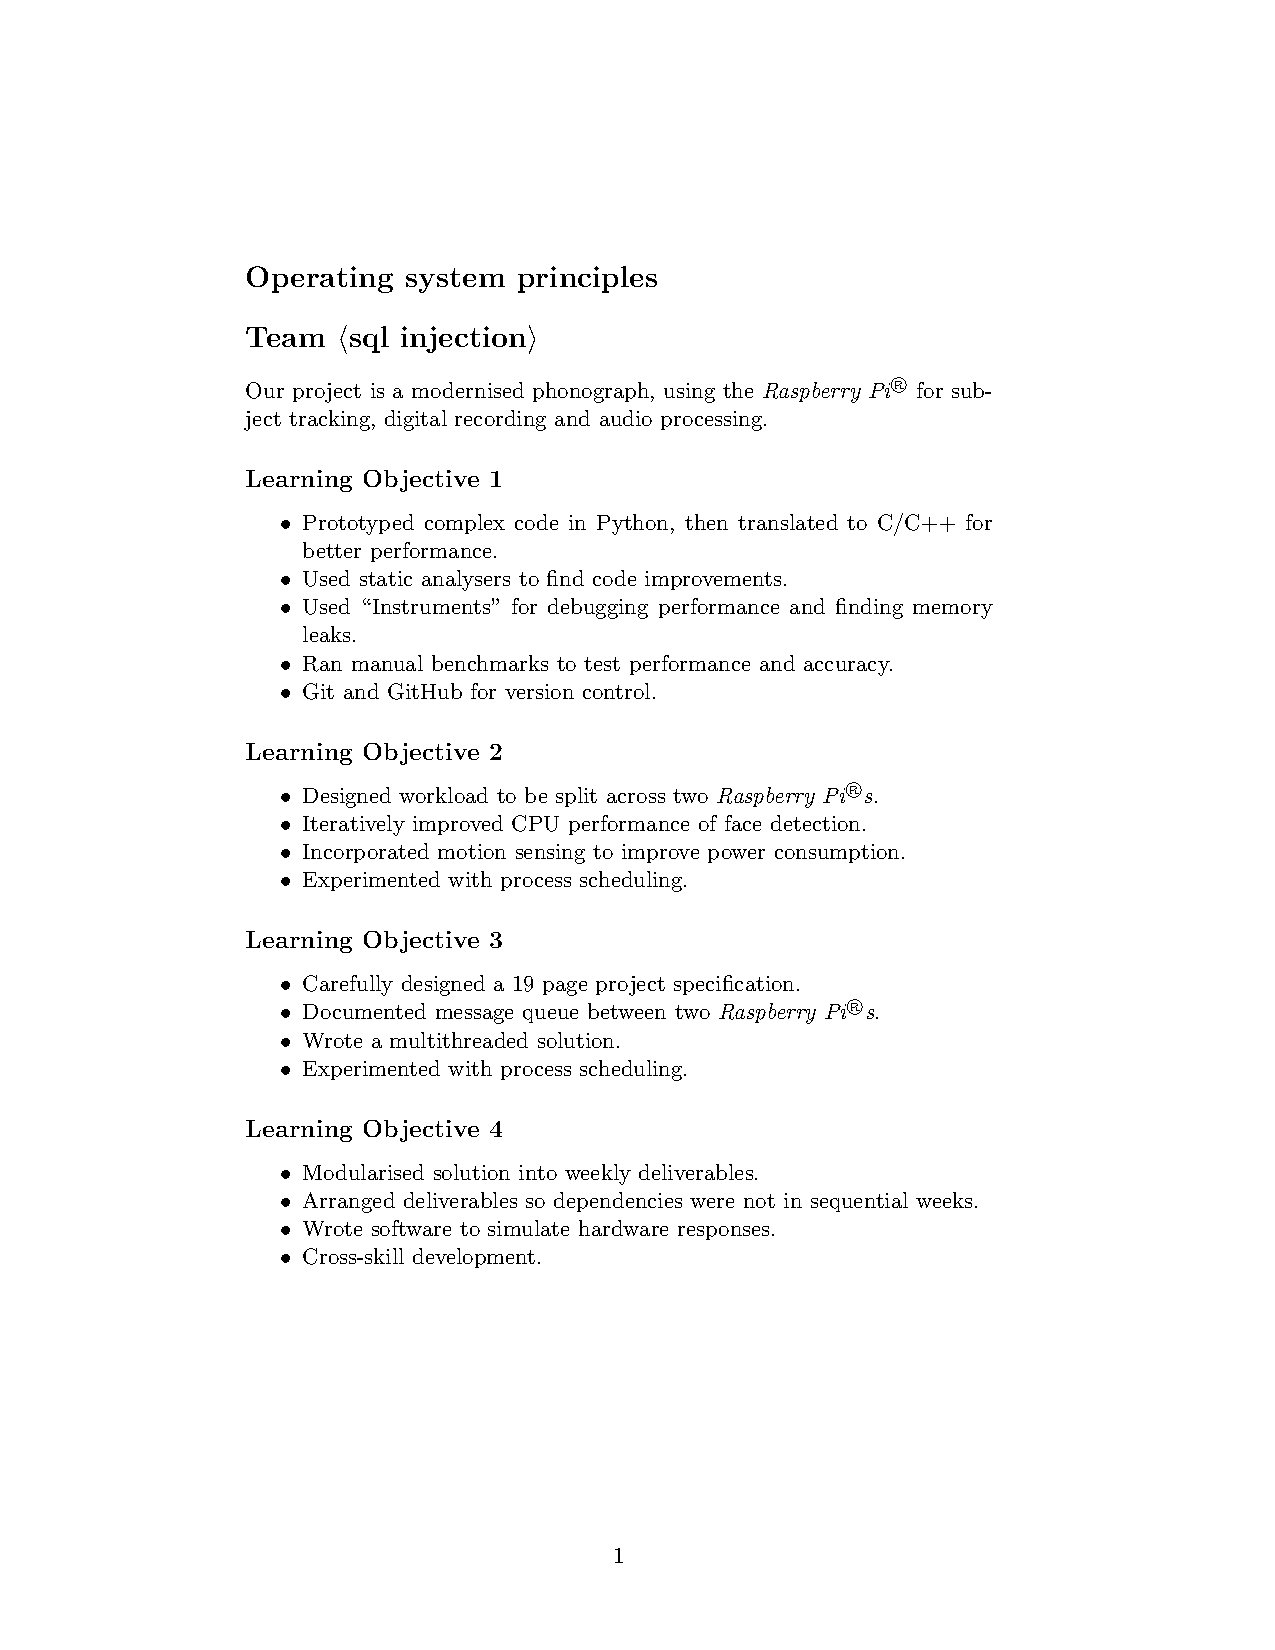
\includepdf[pages=-]{appendix/summary.pdf}



\chapter{Prototype Demonstration - Slides}
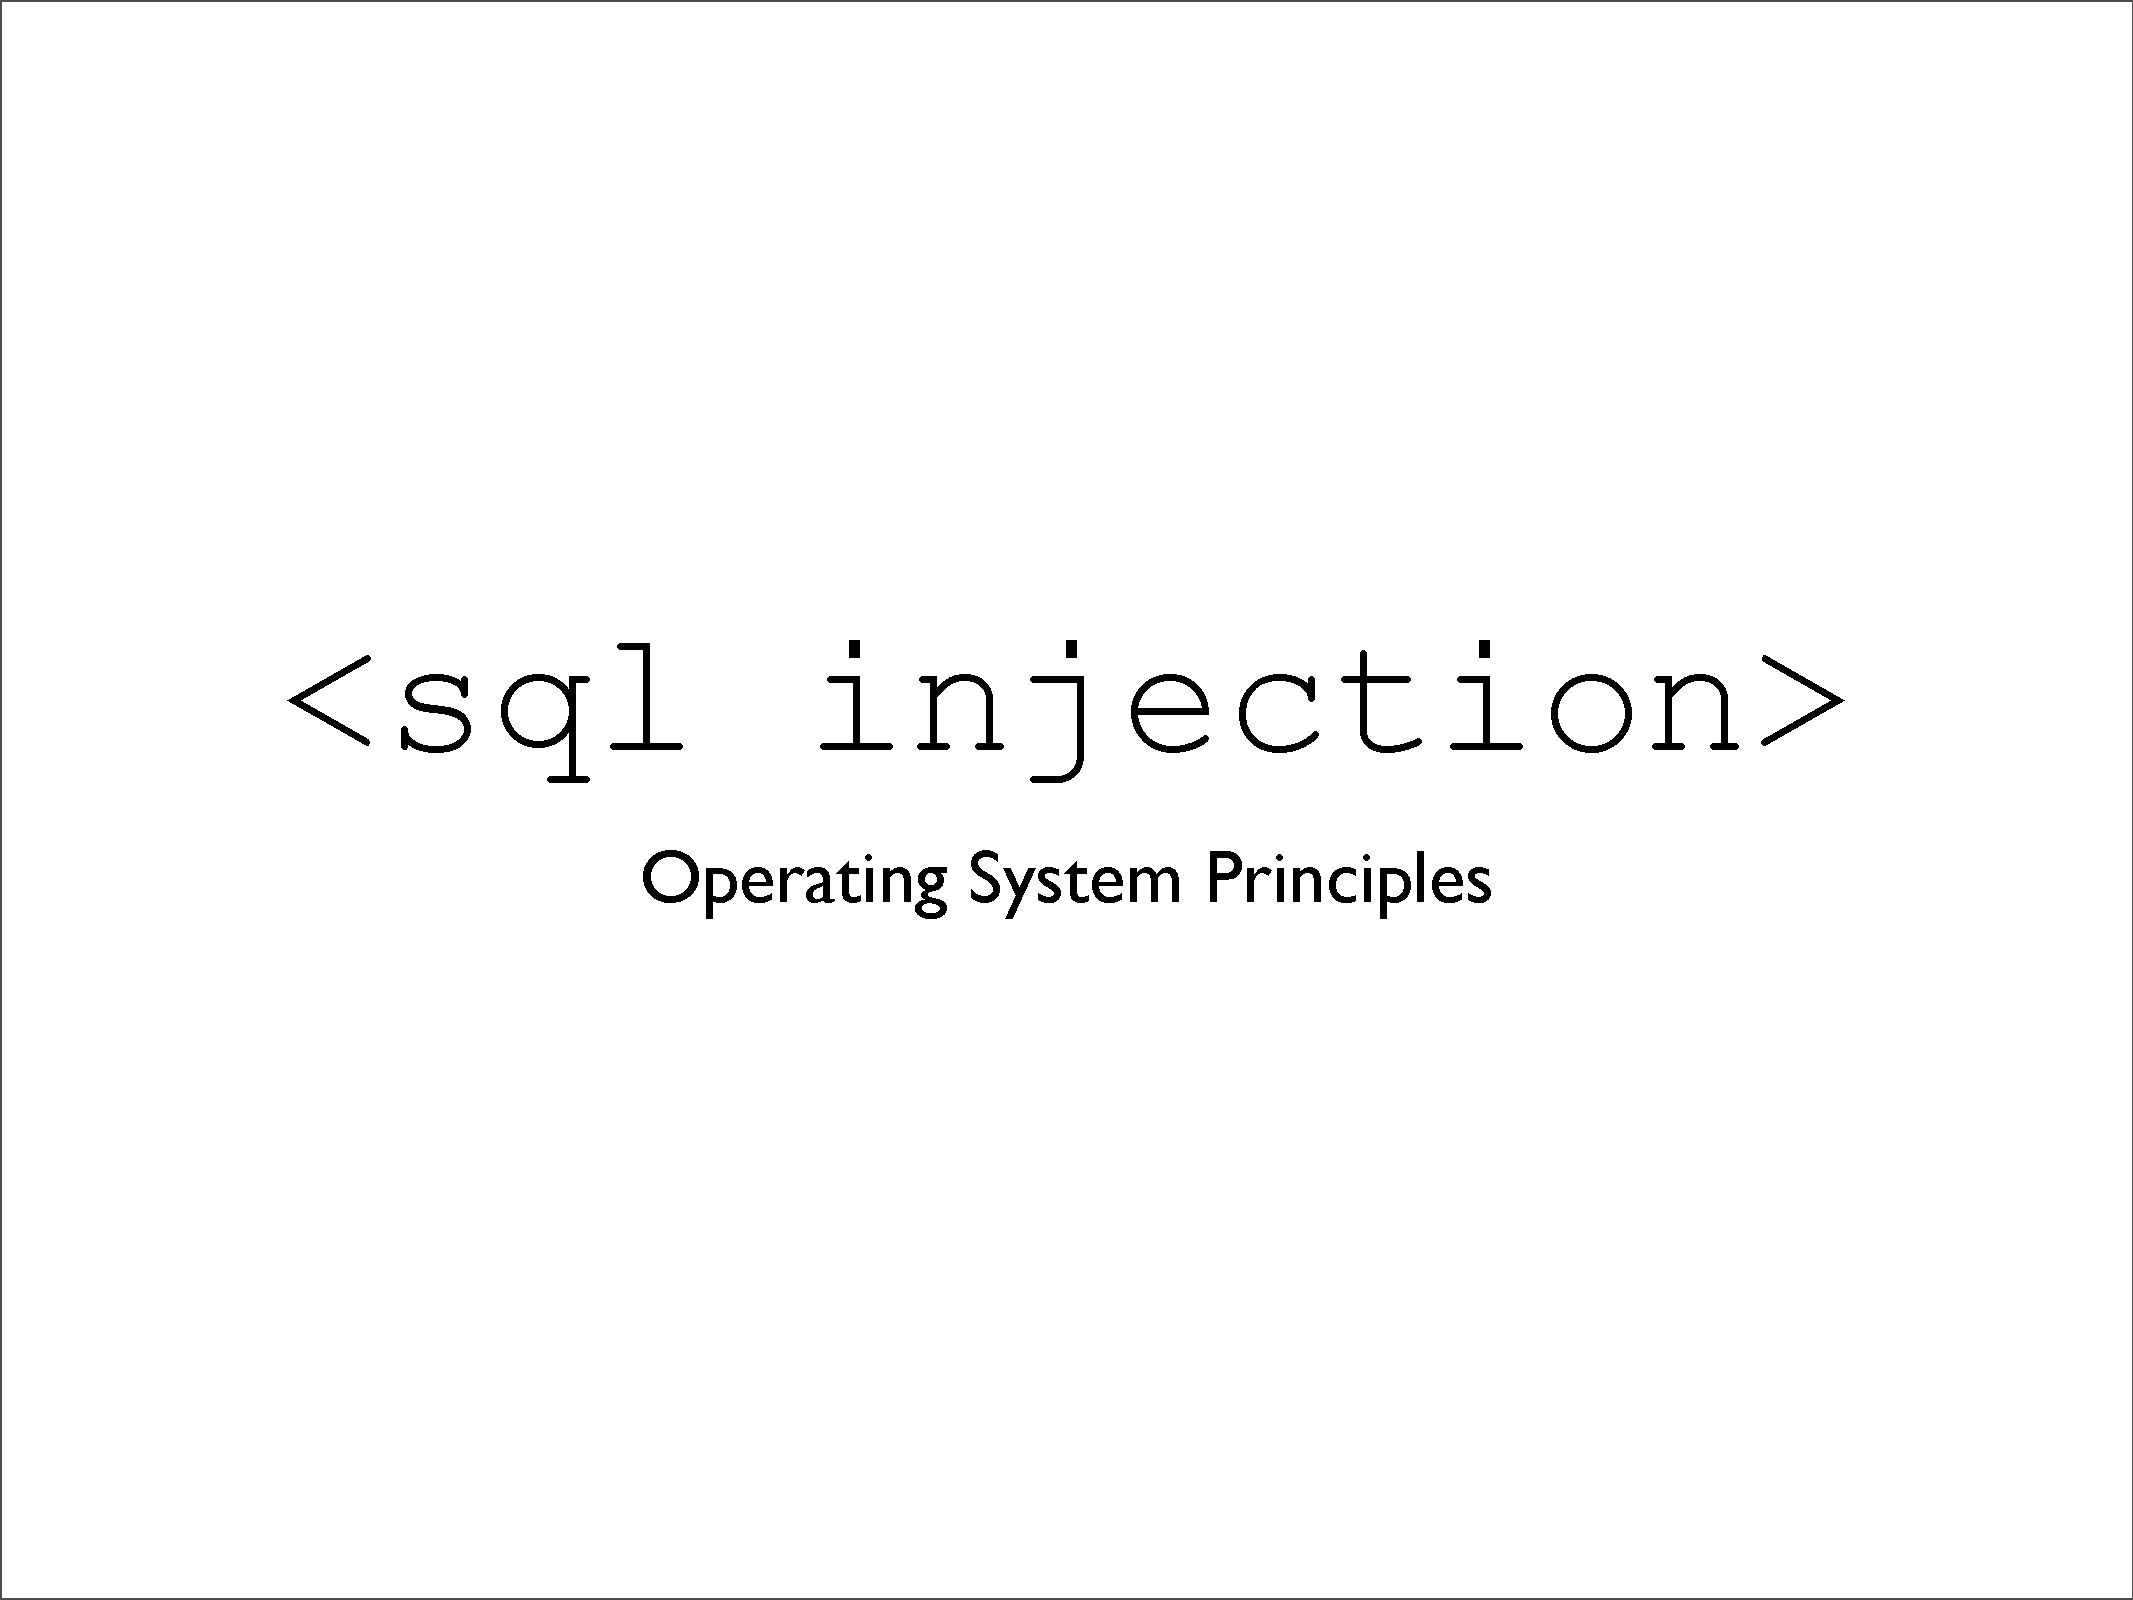
\includepdf[fitpaper=true,pages=-]{appendix/presentation.pdf}


\chapter{Neil's Development Log}
\section*{29th July}

Decided to team up with Val, he is quite experienced in unix and using the raspberry pi, so will compliment my programming skill (and lack of unix and pi skill).

\section*{31st July}

New team member joined the group - Suraj. He has an electronics background and will be helping out with the power work on the project.



\section*{1st August}

My raspberry pi arrived in the mail. Had a bit of trouble scrounging around the house for a SD card. I could only find a 2GB card, and it's not big enough to install Raspbian on, so I installed Arch linux instead. I then ran into trouble because the only USB keyboard I owned is a mechanical keyboard without any keycaps inscription (i.e. blank keys). I am able to touch type, but only in the Colemak layout (not QWERTY). I had to look up each keypress when logging in the first time (it was very slow getting into the pi). I worked out that SSH is setup by default on Arch, so I switched to connecting remotely to it, which was fine.

Our group also decided today to go with the idea to make as smart dictation device with user tracking. Fun times ahead.


\section*{2nd August}

I got the lab cross compile working on the OSP server. Following the instructions made it easy, but I don't think I learnt much about the process of building an image. I had trouble working with tmux, until I learnt you type ctrl-b then the command letter.


\section*{3rd August}

I started researching the OpenCV abilities. I got the libs installed on my laptop (MBP, running OSX). Using Xcode and llvm/clang, I went through the tutorials for OpenCV. I was able to to get face detection working using Haar feature-based cascade classifier for object detection. Face detection was very CPU intensive, so I experimented with reducing frame size and refresh rate to improve CPU performance.

I now need to work out:

\begin{enumerate}
  \item How to make sure it runs smooth on the Pi
  \item How to access the camera on the Pi.
  \item How to deal with multiple faces on screen.
  \item How to smooth face detection so it not "jerky" when working with the servos.
\end{enumerate}

I also had an idea to use hand gestures to control recording start and stop.



\section*{4th August}

New SD card turned up (16 GB), and I was able to get Raspbian installed fairly easily. I wrote up the instruction incase I need to do it again:

\begin{enumerate}

\item Plug your SD card into your MBP.
\item Using Disk Utility, erase the card and set the format to ExFat.
\item Download and unpack the OS image you want to use.
\item Type `df -h` and find the location of the SD card. (If it is `/dev/disk1s1` we will later reference it as `rdisk1`, if it is `/dev/disk2s1` we will reference it as `rdisk2` etc.)
\item In terminal unmount the card: `diskutil unmount /dev/disk1s1`
\item In terminal run: `sudo dd bs=1m if=/path/to/linux-image.img of=/dev/rdisk1`
\end{enumerate}

The default username/password is pi/raspberry.

I spent the rest of the night playing around with Raspbian. I don't have a cam to plug into the pi, so I couldn't test my face detection code. I've ordered an RPi camera from Element14.



\section*{5th August}

Researched using a Microsoft Kinect as an alternative to face recognition. It can measure depth, so it would be better for tracking someone as they move about the room. It would also mean that the program would work in the dark or if the user turned side on. There is an open source project (libfreenect) for interfacing with the Kinect in C++. I found an OpenNI library that can be used for natural interaction and skeletal mapping. However from what I've read, the Kinect can read camera data, but the Pi is not the powerful to do real time skeleton processing. No longer going to pursue this solution.

Although I don't have a camera yet, I installed the OpenCV libs on the Pi and wrote a Makefile to compile my face detection script. It appears to have compiled fine under G++ (I was using clang++ on my laptop).



\section*{6th August}

Acquired the RPi camera board and tested it out. I installed X11 on my laptop and tried to run X windows over SSH to my laptop. I couldn't get it working. I then setup a VNC server on the Pi, and was able remotely view the Pi desktop. I took some photo stills with the built in RPi camera app and could see the output.

Since the RPi camera board is not a USB camera, it is not natively supported by OpenCV and I couldn't test my face detection code.

I tried downloading the userland scripts from the raspberrypi project to work out how to hack in OpenCV support. I was able to compile the userland libs, but still need to incorporate them into my face detection script. It will be a big job so I will leave it for another night.


\section*{7th August}

Continued work on my using the libs from userland with my face detection code. I also did a bit of research on OpenCV performance best practice. Apparently offloading as much workload to the GPU will enable it to run faster. Unfortunately OpenCV only supports NVIDIA/CUDA GPUs. Found out the Pi has a Broadcom chip and VideoCore IV GPU (which is not compatible with OpenCV). I looked through the code to try and work out if I could some how port OpenCV to work on Pi, however, I have never done any OpenGL before and it looks way out of my depth. While looking through the userland code, I discovered the Multi-Media Abstraction Layer (MMAL) framework, which contains references (in the form of enums) to face tracking. This may be a possible alternative to using OpenCV which will use the GPU.


\section*{10th August}

Got my hands on a USB camera to test the face tracking code I wrote before. It was super slow. The Pi could not process the frames at a reasonable speed. I was checking it over VNC, but I think we will need to find ways to speed it up.

Also received some warnings in the libs that I will need to investigate. e.g. \textit{Gtk-WARNING ***: Locale not supported by C library. Using the fallback 'C' locale. Xlib: extension "RANDR" missing on display ":1.0"}.


I've reduced frame size in the script to 320x240 (from 640x480) and FPS to 4. Processing the image from the USB camera is still very slow. The program captures an image, performs the face check, displays the result (and I'm testing this over VNC) and there is a lot of lag as well as >95\% CPU usage. Since the final project won't need to worry about display, I compiled a version which didn't perform the last step (graphical display) but CPU usage was still >80\%.

I read some suggestions on how to improve face detection on this post. I switched out the cascader to lbpcascade\_frontalface.xml, increased the min face detection size and set the CV\_HAAR\_DO\_ROUGH\_SEARCH flag. CPU performance then increased to about 50\% usage. An improvement, but still not perfect.

I have no idea how to do it, but from what I've read, using the GPU would drastically speed up the face detection. I know OpenCV doesn't natively support it, so I'm going to explore what I can do in this space next.



\section*{11th August}

Val and I made the hard decision of dropping Suraj as the third member of our group. After repeated failed attempts to get updates on the progress of his assigned tasks (which was clear he hadn't been working on), we thought it would be best for him to find a new group than stay with us and be down voted for not contributing. We now have the hard task of finding a replacement (most students have already joined new groups).


\section*{12th August}

Since Val and I had not registered a full group, we were both re-allocated to different groups. I went and saw the head tutor during his appointment hours to try and resolve this issue. The plan is for us to make a plea with the other re-allocated groups for a swap.

I sent a message out to the other members, to see if they would like to join our group:

\blockquote{
Hi fellow OSP student,

Val Lyashov and I are postgraduate students who have been working on the assignment since week 1. However, due to an unfortunate accident we've both been reallocated into separate groups.

I've spoken with the head tutor Peter, and he has allowed us the option to switch with a member from our allocated groups so we can continue with the work we've already started together.

For our project we combining computer vision and audio to create a cool new product, and it will also meet the learning objectives. It's an ambitious project, but we have already made significant progress and purchased the required hardware.

Val and myself are both hard working and talented students who are willing to put in the extra hours to get a HD on this project. We are looking for a third member who also determined to do well, and will put in the work that is required. Ideally someone with good technical writing skills would compliment our group best, but anyone who believes themselves to be a hard worker would be fine.

So if you think you would be interested in joining us, or if you have any further questions, please contact me ASAP. We only have until this Wednesday to try and make this work.

Cheers,

Neil Ang
}

We received a response from a student interested in joining, and another student who was facing a similar situation with their group.



\section*{13th August}


I've taken a hiatus from working on the project until the group situation is sorted out. No point continuing with my work if the group has been dissolved.

\section*{14th August}

We acquired a replacement group member, and I am working with Val again. Alfred is the new member and has strong skills with C/C++. He will make a good addition to the team and helpful with writing the low level C code that interfaces with the hardware. We caught him up to speed on the project and re-assigned tasks.

We attempted the demonstrated the Cross compile milestone to the lab instructor, but because Alfred was new he hadn't completed the work. We will try again next week.

\section*{17th August}

Since Alfred strongest skill is in programming, and Val in unix/hardware, I've taken over responsibility for the documentation. Started work on the project specification. Using LaTeX to give it a professional presentation. Also organised a group meeting for next Tuesday.


\section*{18th August}

Continued work on project specification. As I'm the only one working on it, it will take a long time to write up.

\section*{20th August}


Had our group meeting, everything feels on track. I demonstrated the work I had done with OpenCV, and gave Alfred instructions on how to continue on with the work I started. He will be looking at integrating the RPi camera board with my face detection script.

To help Val work on his servo controller, I wrote a small C++ script to imitate coordinate output by the face detection code without needing to run a camera. It will put out a random x and y position, pause and then output another coordinate within a specified tolerance (to mimic natural movement). I've noticed my C++ programming skills are improving. I also continued work on the project specification.

\section*{21st August}


Had our class tutorial and demonstrated the teams cross-compile. It worked, so we have passed the first milestone. As a group we spent some time discussing the program architecture. I'm going to do some research into pi-to-pi communication. Val suggested we could use a message queue over TCP or UDP so I will investigate that this weekend.

We also had a discussion how the servos will respond to face detection. We can't capture depth so the servo won't accurately know how far to tilt in each direction. What we decided to do is have the servo move a little bit in the direction of the face (we will experiment to get a magic number), then re-evaluate the face position and move again. We also decided we will need a "seeking" or "hunting" mode on the project to search the room for a face when none can be found. It's not going to be easy.

I spent the rest of the time updating the project specification. It is about a third finished.

\section*{24th August}


Updated the test face detection script to output numbers in a different range. I also worked on the project specification.

\section*{26th August}


Added more content to the project specification. Cancelled our weekly group meeting (scheduled for tomorrow), as there is nothing new to demo between the members.

\section*{30th August}

Worked hard to get the project specification finished. It was submitted successfully on time.


\section*{8th September}

Started work on porting pir-monitor from Python to C. First I started reading up on connecting the PIR. The sensor we will be using is the "SEN-08630". It has 3 wires to connect it: power, ground and alarm.

"Red wire is power (5 to 12V). Brown wire is GND. Black wire is open collector Alarm.

The alarm pin is an open collector meaning you will need a pull up resistor on the alarm pin. The open drain setup allows multiple motion sensors to be connected on a single input pin. If any of the motion sensors go off, the input pin will be pulled low." - \url{http://littlebirdelectronics.com/products/pir-motion-sensor}

The first issue I ran into with this was how to physically connect the PIR sensor to the Pi. I realised I didn't have the correct cables to join them, so I drove down to Jaycar to buy a male-female jumper wire. Jaycar don't sell these cables, but showed me what parts I would need to build my own breakout board. I purchased a 26 pin connector, 1 metre of ribbon, a copper board and mini breadboard. I tried connecting them together but broke the pin connector. Feeling like I war running out of options, I contacted Val who invited me around to his place to borrow some of his jumper wires.

With the sensor connected I tried running Val's python script. It worked well.

I did a bit of research and found out there are two forms of pin monitoring I could use: polling and interrupts. Obviously interrupts would be the better option, but there is limited support from C libraries for this.

After some more reading I found a C library written for the RPi chip (the lib is called bcm2835). I then wrote a C implementation of the Python code using this lib. It worked first time without issue. I played around with the delay when polling the sensor for movement, I found that event with a delay of only 33ms the CPU usage was really low (i.e. <1\%).




\section*{10th September}

Read up on IPC techniques, to see if we could use named pipes that were covered in class as a way to have our processes talk to each other. It appears that UNIX domain sockets could be a better option, if we were to use processes instead of threads.

I also did a bit of research into using interrupts with the GPIO pins on the Pi. Seems that the newer OS versions support it, but it also looks more complex to implement. My thoughts now are that the C-based pir-monitor code is already very efficient (<1% cpu) and that it would be overkill to optimise at this point.




\section*{11th September}

Today Val gave me the servos and mount he had been working on, and I'm going try and rewrite it to work in C/C++ as well as integrate it with the face detection program.

The device is a "Pololu Maestro Servo Controller". I found a sample C script (\url{http://www.pololu.com/docs/0J40/5.h.1}) for interacting with the device and tried to run it with it plugged into my MBP.

However I got the error: \textit{"/dev/cu.usbmodem00034567: No such file or directory"}

I had a look under /dev and couldn't find the device. I started reading up on /dev (here: \url{http://www.linuxjournal.com/article/2597}) to learn more about this directory and see if I was doing anything wrong. I didn't find any helpful answers.

I returned to the manufacturers website and found this \textit{"We do not provide any software for Mac OS X, but the Maestro’s two virtual COM ports are compatible with Mac OS X 10.7 (Lion) and later."} Which made me think that it must be possible. I started up a VM running OS X 10.7 (I'm using 10.8) and looked for the /dev/cu.* devices. None.

After more googling I realised that I had powered on the device with the provided battery, but not connected the USB cable (rookie mistake!!). As soon as I plugged it in the two devices appeared "/dev/cu.usbmodem00065291" and "/dev/cu.usbmodem00065293". These were different from what was expected from the manufacturers instructions, but using "/dev/cu.usbmodem00065291" worked with the script. I'm assuming two devices appeared because we have 2 servos connected.

With it now working I tried running the python test scripts that Val had added to the repository. Unfortunately I had trouble running them on my machine and debugging them was difficult as I'm not experienced in python. So I thought I should try setting them aside and re-programming in ruby first (to learn how the device works), then optimise in C. Val had done some great work to get it running in Python, but being a professional ruby programmer I feel more comfortable approaching something new with a familiar language. I found a gem someone had started which looked promising (\url{https://github.com/adammck/pololumaestro}), but after downloading it and inspecting the source it appeared to be half finished and not functioning. If I have time remaining in this project, I will try and fix up the gem and send a pull request, but for now I need to get this working.




\section*{15th September}


Reading up on servo controller. The two /dev ports are not because of the two USBs, but two different ports \textit{"the Maestro shows up as two virtual serial ports on a computer if it is connected via USB. One of these ports is called the Command Port and the other is called the TTL port."} (Source: \url{http://www.pololu.com/docs/0J40/5.a}).

I Loaded up a VM of Windows so I could run the Pololu system settings application. I used the manufacturer application to verify that the all the hardware was working.

Val came around to my place to work on the project. I found out battery was not connected to the servos correctly which was causing all my issues with the code. The original test code I wrote earlier worked all along.

Talking with Val I found out on Raspberry Pi I can reference the port like so: /dev/serial/by-path/platform-bcm2708\_usb-usb-0:1.2.2:1.0. Also if the servo controller is flashing yellow is "awaiting command" and a bright red light means there is an error. Errors need to be cleared before continuing.

After a bit of "brute forcing" we worked out the pivot range of the servos. We tried combining the moving code with the face detect code, but it didn't work perfectly. It needs refinement.

While testing out the servo the battery cables physically broke. Val took the battery jack home to re-solder. After it was repaired it still didn't seem to work. Current theory is that the connection is still broken or the battery power is low.



\section*{16th September}


I recharged the batteries for the servo controller and it didn't work. To see if it was the battery jack I thought I would try a different power source. Val told me earlier today that the servo controller needs 5V of power, but it can't come from the Raspberry Pi because it draws too much and the hardware will reset. I own an Arduino and remember it had a 5V pin. I plugged that into my computer and used to jumper wires to connect it the servo controller. Success! It was working again. It turns out the battery jack isn't working at all.

Started to write a C++ based interface for communicating with the servo controller. Ran into to some trouble trying to use pure C++ and online posts suggest that I have to drop down to C to communicate with a device (e.g. \url{http://stackoverflow.com/questions/6064890/reading-a-linux-device-with-fstream}).

I wrote a C++ class that would do some basic interaction:

\begin{lstlisting}[language=C++]
int goHome(unsigned char);
int getPosition(unsigned char);
int setPosition(unsigned char, unsigned short);
bool isMoving(unsigned char);
\end{lstlisting}

Since the servo takes a few seconds to get into a position, I wrote a special busy wait function to constantly query the servos.

\begin{lstlisting}[language=C++]
void busyWait(Maestro *maestro, unsigned char channel){
    while(maestro->isMoving(channel)){
        usleep(100000);
    }
}
\end{lstlisting}

It works ok, but if a position is set on the servos that they can't reach, this function will never complete... hmmm.




\section*{17th September}

Kept working on my C++ wrapper for controlling the servo. I added a new "Servo" class to model the two individual servos in the library. I made them classes, but they could easily be replaced as structs.

I also came up with a method for detecting a busyWait lock that I was seeing yesterday. The fix is to use the last recorded position to detect if the servo is still moving between sleeps:

\begin{lstlisting}[language=C++]
void busyWait(Maestro *maestro, Servo * servo){
    int pos = maestro->getPosition(servo);
    while(maestro->isMoving(servo)){
        usleep(100000);
        if(maestro->getPosition(servo) == pos){
            break;
        }
        else {
            pos = maestro->getPosition(servo);
        }
    }
}
\end{lstlisting}

I also copied in some code into my example library to detect key presses. It was fun to use the keyboard to play around with moving the servos. I tried adding the camera mount but soon worked out that the mount had a bad effect on the servos reaching their programmed positions. I removed the mount and use some garden wire to fasten the camera to the servos. It doesn't look pretty but it overcomes the issues so I can continue testing.




\section*{22nd September}

We have obtained a new battery pack and lighter camera mount. Unfortunately one of the screws have come loose on the bottom servo, so I will need Val's assistance to fix it.

I've been looking into a technique to work out intersecting shapes in C++. Previously in objective-c I've used the CGGeometry framework which has a lot of convenient methods to determine intersecting shapes. However, in C++ I can't find any reference to a standard Rect struct or shape based math functions. I find it hard to believe that C++ would not have this. After a bit of googling I found out that OpenCV has a rect struct implementation. Instead of writing my own I will just look at re-using it (\url{http://docs.opencv.org/modules/core/doc/basic_structures.html#Rect_}).

Val came around to my place to work on the assignment. We connected up a new battery pack to the servos, but for some reason they made the movement very choppy.

We also wanted to build a stronger mount to hold the servos down, so we took a trip down to Bunnings and got some timber cut and bought some metal brackets. After a bit of fiddling we had the mount built. There was a bit of an issue with the microphone appearing in the camera frame, so had to position it back and a little offside.

I updated my C++ code to respond to the faces position. It was very simple. It would take the center point on a persons face then shift the servos in the direction that would make is more center. I ran the code on my MBP first, and it worked fantastic.

We took some audio samples and found that the servo movement could be heard in the background of the recording. We also tried sending the recordings to a speech translation service. The translations we got back were not great. They were very inaccurate. We tried our experiments again, but spoke with an American accent the second time. The translations improved but were still off.

The next thing we did was to try and run the face tracking code on the Pi. We had issues. The servo controller kept returning a strange error, and the face detection was slow. I tried debugging it, but nothing seemed to work. I will have to go through it line-by-line to work out the issues.

\section*{23rd September}

I spent hours tonight trying to debug my servo interface on the Pi. The code I wrote works perfectly on OS X, but not on the device. Which is strange because it is using standard C++ calls. Writing to the serial port is fine, but trying to read from it hangs. I tried modifying small bits of the code at a time to see if they would make a difference, but nothing seems to work. The weird thing is that reading from the device causes it error, but to get the error value you need to do another device read. I'm a little lost as to what to try next. I can rewrite my code to not use reads, but I think that should be a last resort.


\section*{24th September}

Took the whole day off work to meetup with the team at RMIT and work on the project. Unfortunately we couldn't get a meeting room because they were all booked out. After wandering around for a bit we setup shop in a student common room. The amount of cables and wires we need to plug in to make this work together caused a bit of mess.

I spent the day trying to further debug the servo issue. After wasting a few hours I decided to go with plan B and stop performing 'reads' on the servo controller. What this means is that we can't use the 'busyWait' function I developed earlier, and just have to assume the servo reached its destination. I re-wrote the code to do this and put on GitHub.

I then re-combined my simple face detect code to work with the servos. I spent a lot of time testing and fine-tuning the stepping values for moving the camera towards the centre.

While testing I occasionally ran into an issue where the camera would receive a false-positive face detection in the background and shift away from the user. Because we were working on a student common room it would lock onto the face of another student in the background. To overcome this I came up with the idea of measuring the Euclidean distance from the last face position compared to the new one. This way if a false-positive was detected it wouldn't shift in that direction immediately. It could check to see if the face occurred within a close proximity of the last known face position, which yielded a surprising positive result. The subject tracking responded generally more smoothly after implementing this. If a subject was to suddenly move beyond the Euclidean threshold, the servos would still shift to that position but it takes an extra pass to update the last detected position before moving.

I then worked with Alfred to implement his faster threaded face detection code. It didn't respond as well as on the MBP, but was still reasonable. Alfred had some new ideas to improve the face detection even further, by only scanning for faces in the last known position first. He is going to continue the work on this, so we gave him the servos to take home after the meeting.


\section*{28th September}

The team met together again to work on the solution for the whole day. Because we want the system to automatically startup when turned on I worked on writing a daemon script. I spent the morning reading up on how daemons can work, and how I could write a self starting script that would keep a process alive, or at least restart it if it quit unexpectedly.

So I started working on a C script that would run in the background, spawn a child deamon that could monitor another process and restart it if it quits. I found a lot of helpful information on the topic here: \url{http://www.netzmafia.de/skripten/unix/linux-daemon-howto.html}

On my first attempt I managed to write a 'fork bomb' that kept spawning children processes unchecked. I had to restart my machine to regain control of it. On my second attempt I wrote some code that would fork itself, then if it quit it would fork two more of itself and kept doubling. Closer but still not good.

I eventually got the code working correctly:

\begin{lstlisting}[language=C++,caption=daemon.c]
// Based off: http://www.netzmafia.de/skripten/unix/linux-daemon-howto.html
#define EXE "/Users/neil/Desktop/beeps"

#include <sys/stat.h>
#include <stdlib.h>
#include <unistd.h>
#include <signal.h>

int main(void) {

    pid_t pid, sid;

    /* Fork off the parent process */
    pid = fork();
    if (pid < 0) {
        exit(EXIT_FAILURE);
    }
    /* If we got a good PID, then
     we can exit the parent process. */
    if (pid > 0) {
        exit(EXIT_SUCCESS);
    }

    /* Change the file mode mask */
    umask(0);

    /* Open any logs here */

    /* Create a new SID for the child process */
    sid = setsid();
    if (sid < 0) {
        /* Log the failure */
        exit(EXIT_FAILURE);
    }

    /* Change the current working directory */
    if ((chdir("/")) < 0) {
        /* Log the failure */
        exit(EXIT_FAILURE);
    }

    /* Close out the standard file descriptors */
    close(STDIN_FILENO);
    close(STDOUT_FILENO);
    close(STDERR_FILENO);

    /* Daemon-specific initialisation goes here */
    while (1) {
        pid_t cid;

        /* Create a child process */
        cid = fork();

        if (cid == 0) {
            /* Replace child process with other program */
            execv(EXE, NULL);
            exit(EXIT_FAILURE); // this will never be reached
        }
        else if(cid < 0) {
            /* Handle child create error */
            exit(EXIT_FAILURE);
        }

        /* Wait for child process to die */
        waitpid(cid, NULL, 0);
        sleep(2);
    }

    exit(EXIT_SUCCESS);
}
\end{lstlisting}

With that written I sent it to Val to integrate.

I then talked to Alfred about the response speed with face detection and movement. Because it was running slower on the \rpi \xspace I had an idea to use trigonometry to make smarter position shifts. The theory was that because we can detect the face 'width' we could use that information to make rough guesses as to the depth of the face. e.g. A face that was closer would be wider and our servos would have to shift more (i.e a larger number of steps) when reposition to the centre, whereas a face a few metres back would be narrower and the servos would have to shift less to get them centred. I spent a good 2-3 hours working on this problem but found the math to be too difficult and the shifting would require a lot of time to come up with the right magic numbers to insert into the shifting formula.


\section*{29th September}

The very next day the group got together again to work on the project. We won't get a chance to meet before our lab demonstration so we treated the project as though it was due that day. We all worked hard to finish off our parts. 

I spent most of the days writing a speech and slide show to give in Wednesday's lab. I also shot a backup video incase we ran into any problems and the product stopped working. I also created a one pager as a handout for the class.

\section*{2nd October}

Today was demo day. A few hours before the demonstration we found an issue with the project. If the hardware wasn't connected in the right order during startup it would crash. Alfred and Val got together 20 mins before the lab was meant to start and quickly patched the issue. 

Our project was the second demonstration and was very well received by our peers. There were no technical hiccups and a lot of interest in the project from everyone. After the class a great sense of accomplishment came over us, and we were very proud of what we had made. We celebrated by going to the pub.

Since the project was technically working, we decided to spend the remanding weeks focusing on producing the portfolio.

\chapter{Val's Development Log}
\section*{15th August}

\begin{itemize}
  \item received replacement external soundcard as the initial one was DoA (guess for\$3 dollars can't really complain). No problems using the bcm2835 kernel module. The following steps enable the card at init \url{http://www.linuxcircle.com/2013/05/08/raspberry-pi-microphone-setup-with-usb-sound-card/}.
  \item I increased the gain to +11db , otherwise a bit too quite for lecture recording.
  \item Encountered a lot of noise during recording which seems to be a biproduct of lack of shielding/circuit isolation on the Pi. Moving the device to a usb hub seems to have improved things though still sounds like clipping at the top end. Will keep trying.
  \item Lastly, finally got around to expanding the available root partition space with parted.. now have additional 13gig for sound storage. Instructions found here \url{http://www.raspberrypi.org/phpBB3/viewtopic.php?f=51&t=45265}
  \item Updated the test script to run 2 servos connected via the gpio pins, using software controls
prototype setup of 2 servos
\end{itemize}


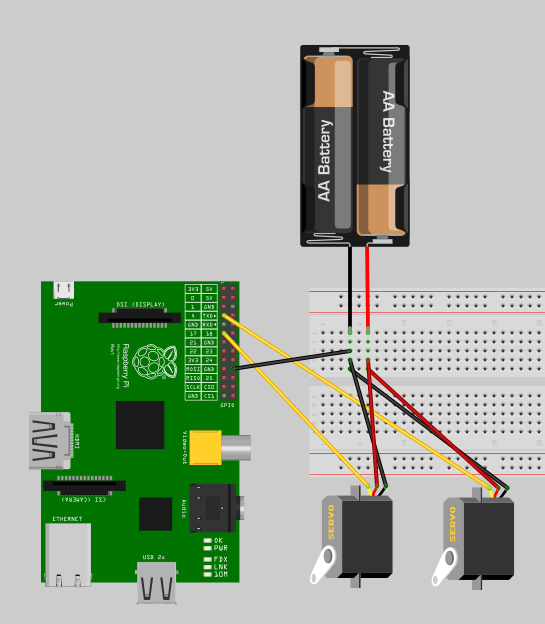
\includegraphics[width=\textwidth]{graphs/proto2.png}

\section*{18th August}

\begin{itemize}
  \item Completed assembling the usb servo controller and added pin connectors to power block and mechanical switch
  \item Tested out the PIR sensor, sample scripts uploaded including one with a on/off switch activation
  \item Got the pololu servo controller working over the USB virtual serial port, starting working on easing using the speed control... not sure if would use it though
\end{itemize}



\section*{19th August}

\begin{itemize}
  \item Put together a script for communicating with the Pololu servo over the USB serial port. Setting acceleration param does easing automatically which is pretty handy if we are going to do video recording at the same time as record.
  \item Still looking for a suitable base plate to attach to the Y servo bracket... a bit worried of whether the plastic gearing I have on X servo can handle the extra weight... may have to pick up a large metal gear from a hobby store if it starts to slip once the mic and camera are mounted on it.
  \item Starting to work on networking 2 RPis and whats an efficient (read: basic + lowest overhead) coms channel we can use for issues commands over.
\end{itemize}



\section*{30th September}

\begin{itemize}
  \item Creating a systemd service to launch the server (master) daemon...
    \begin{itemize}
      \item groupadd osp \# create a new group
      \item useradd -r -g osp osp \# create a system account osp in the new group
      \item chown osp:osp /usr/local/bin/osp\_server \# set ownership of the daemon
      \item add the service script (in src dir) to /etc/systemd/system/
      \item systemctl daemon-reload \# reloads the available services descriptions
      \item systemctl start osp-project.service \# to start the service straight away
      \item systemctl enable osp-project.service \# get the service to start at boot-time
    \end{itemize}
  \item Added a wireless interface to connect to backup router for maintenance config (network-wireless.service in src dir). Like before, systemctl daemon-reload/enable ...

\end{itemize}



\chapter{Project Specification}
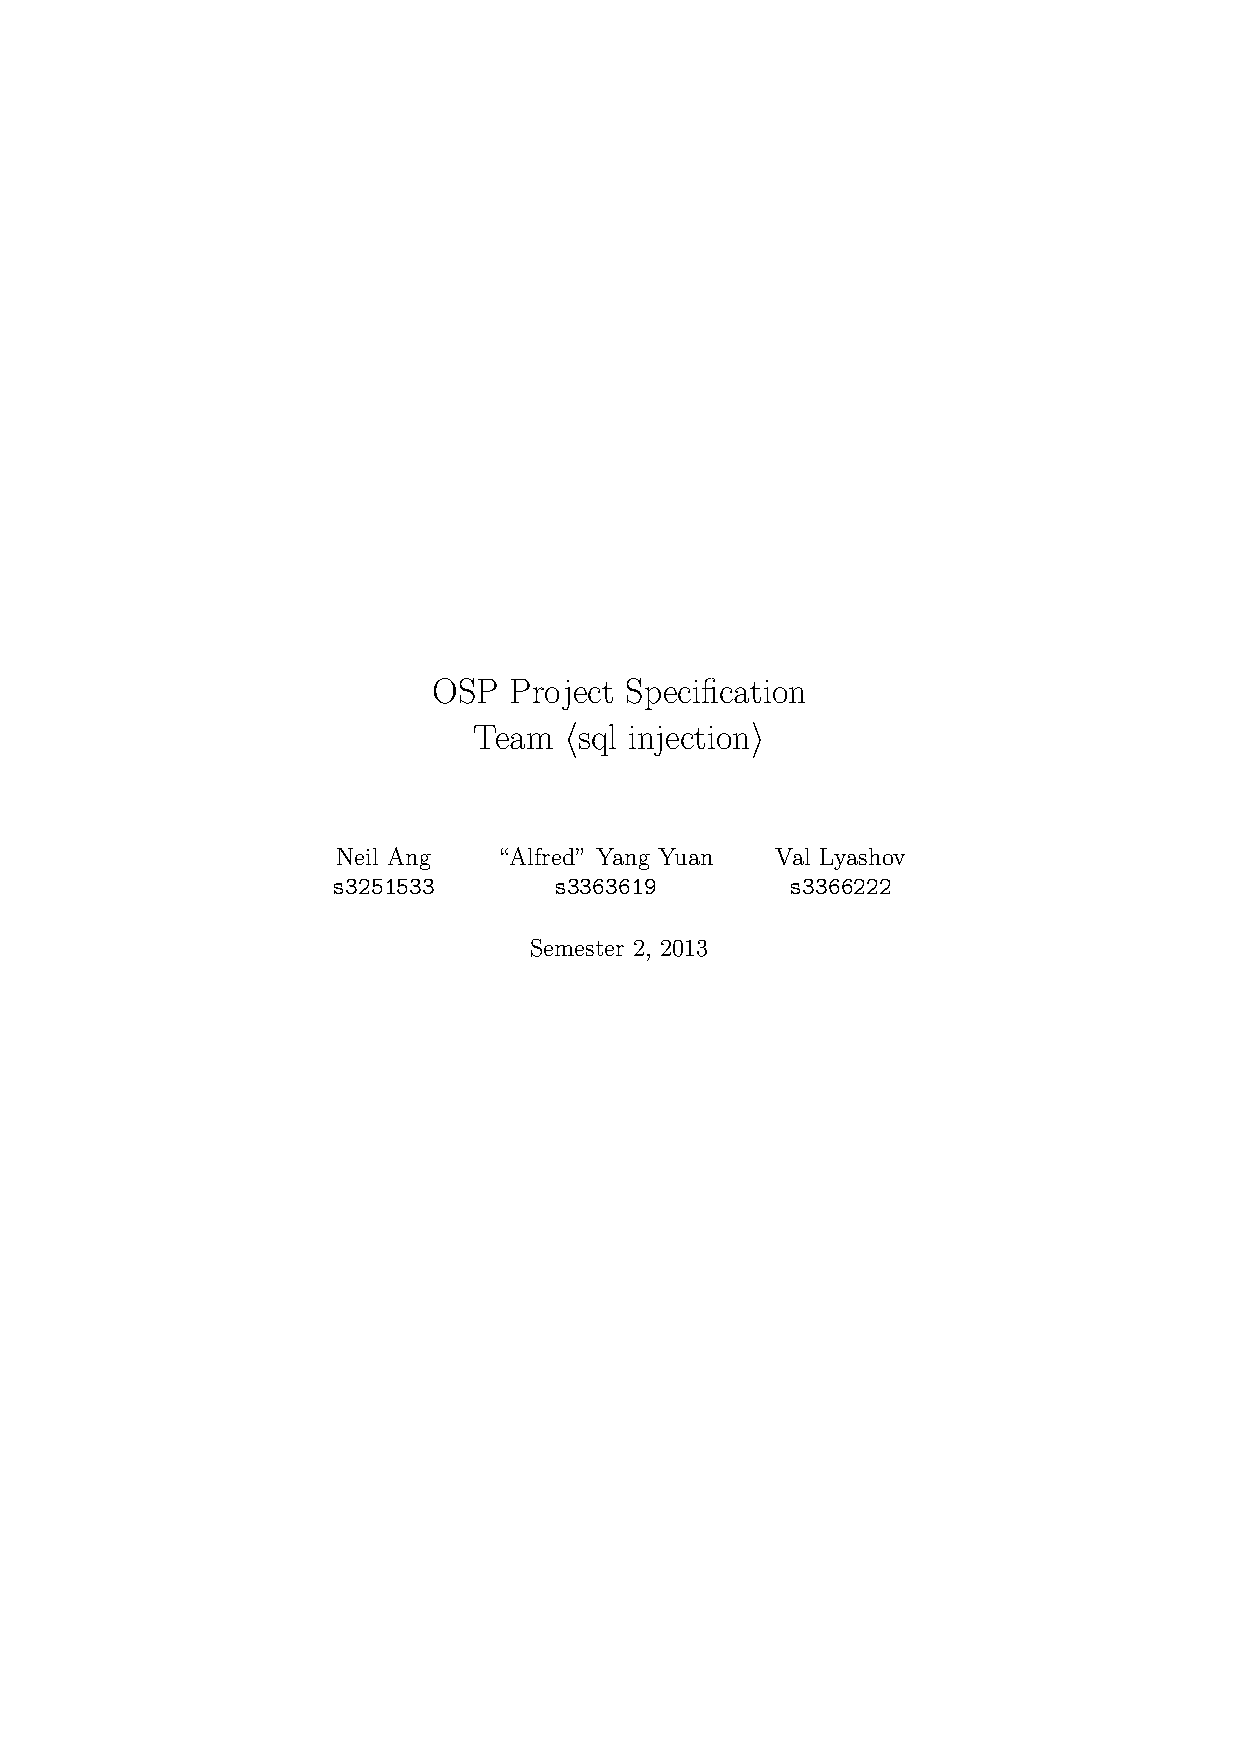
\includepdf[pages=-]{appendix/specification.pdf}



\end{appendices}

\nocite{*}
\printbibliography[heading=bibintoc]


\end{document}